% Options for packages loaded elsewhere
\PassOptionsToPackage{unicode}{hyperref}
\PassOptionsToPackage{hyphens}{url}
\PassOptionsToPackage{dvipsnames,svgnames,x11names}{xcolor}
%
\documentclass[
  11pt,
]{article}

\usepackage{amsmath,amssymb}
\usepackage{iftex}
\ifPDFTeX
  \usepackage[T1]{fontenc}
  \usepackage[utf8]{inputenc}
  \usepackage{textcomp} % provide euro and other symbols
\else % if luatex or xetex
  \usepackage{unicode-math}
  \defaultfontfeatures{Scale=MatchLowercase}
  \defaultfontfeatures[\rmfamily]{Ligatures=TeX,Scale=1}
\fi
\usepackage{lmodern}
\ifPDFTeX\else  
    % xetex/luatex font selection
    \setmainfont[]{Times New Roman}
\fi
% Use upquote if available, for straight quotes in verbatim environments
\IfFileExists{upquote.sty}{\usepackage{upquote}}{}
\IfFileExists{microtype.sty}{% use microtype if available
  \usepackage[]{microtype}
  \UseMicrotypeSet[protrusion]{basicmath} % disable protrusion for tt fonts
}{}
\makeatletter
\@ifundefined{KOMAClassName}{% if non-KOMA class
  \IfFileExists{parskip.sty}{%
    \usepackage{parskip}
  }{% else
    \setlength{\parindent}{0pt}
    \setlength{\parskip}{6pt plus 2pt minus 1pt}}
}{% if KOMA class
  \KOMAoptions{parskip=half}}
\makeatother
\usepackage{xcolor}
\usepackage[margin=2.5cm]{geometry}
\setlength{\emergencystretch}{3em} % prevent overfull lines
\setcounter{secnumdepth}{5}
% Make \paragraph and \subparagraph free-standing
\makeatletter
\ifx\paragraph\undefined\else
  \let\oldparagraph\paragraph
  \renewcommand{\paragraph}{
    \@ifstar
      \xxxParagraphStar
      \xxxParagraphNoStar
  }
  \newcommand{\xxxParagraphStar}[1]{\oldparagraph*{#1}\mbox{}}
  \newcommand{\xxxParagraphNoStar}[1]{\oldparagraph{#1}\mbox{}}
\fi
\ifx\subparagraph\undefined\else
  \let\oldsubparagraph\subparagraph
  \renewcommand{\subparagraph}{
    \@ifstar
      \xxxSubParagraphStar
      \xxxSubParagraphNoStar
  }
  \newcommand{\xxxSubParagraphStar}[1]{\oldsubparagraph*{#1}\mbox{}}
  \newcommand{\xxxSubParagraphNoStar}[1]{\oldsubparagraph{#1}\mbox{}}
\fi
\makeatother

\usepackage{color}
\usepackage{fancyvrb}
\newcommand{\VerbBar}{|}
\newcommand{\VERB}{\Verb[commandchars=\\\{\}]}
\DefineVerbatimEnvironment{Highlighting}{Verbatim}{commandchars=\\\{\}}
% Add ',fontsize=\small' for more characters per line
\usepackage{framed}
\definecolor{shadecolor}{RGB}{241,243,245}
\newenvironment{Shaded}{\begin{snugshade}}{\end{snugshade}}
\newcommand{\AlertTok}[1]{\textcolor[rgb]{0.68,0.00,0.00}{#1}}
\newcommand{\AnnotationTok}[1]{\textcolor[rgb]{0.37,0.37,0.37}{#1}}
\newcommand{\AttributeTok}[1]{\textcolor[rgb]{0.40,0.45,0.13}{#1}}
\newcommand{\BaseNTok}[1]{\textcolor[rgb]{0.68,0.00,0.00}{#1}}
\newcommand{\BuiltInTok}[1]{\textcolor[rgb]{0.00,0.23,0.31}{#1}}
\newcommand{\CharTok}[1]{\textcolor[rgb]{0.13,0.47,0.30}{#1}}
\newcommand{\CommentTok}[1]{\textcolor[rgb]{0.37,0.37,0.37}{#1}}
\newcommand{\CommentVarTok}[1]{\textcolor[rgb]{0.37,0.37,0.37}{\textit{#1}}}
\newcommand{\ConstantTok}[1]{\textcolor[rgb]{0.56,0.35,0.01}{#1}}
\newcommand{\ControlFlowTok}[1]{\textcolor[rgb]{0.00,0.23,0.31}{\textbf{#1}}}
\newcommand{\DataTypeTok}[1]{\textcolor[rgb]{0.68,0.00,0.00}{#1}}
\newcommand{\DecValTok}[1]{\textcolor[rgb]{0.68,0.00,0.00}{#1}}
\newcommand{\DocumentationTok}[1]{\textcolor[rgb]{0.37,0.37,0.37}{\textit{#1}}}
\newcommand{\ErrorTok}[1]{\textcolor[rgb]{0.68,0.00,0.00}{#1}}
\newcommand{\ExtensionTok}[1]{\textcolor[rgb]{0.00,0.23,0.31}{#1}}
\newcommand{\FloatTok}[1]{\textcolor[rgb]{0.68,0.00,0.00}{#1}}
\newcommand{\FunctionTok}[1]{\textcolor[rgb]{0.28,0.35,0.67}{#1}}
\newcommand{\ImportTok}[1]{\textcolor[rgb]{0.00,0.46,0.62}{#1}}
\newcommand{\InformationTok}[1]{\textcolor[rgb]{0.37,0.37,0.37}{#1}}
\newcommand{\KeywordTok}[1]{\textcolor[rgb]{0.00,0.23,0.31}{\textbf{#1}}}
\newcommand{\NormalTok}[1]{\textcolor[rgb]{0.00,0.23,0.31}{#1}}
\newcommand{\OperatorTok}[1]{\textcolor[rgb]{0.37,0.37,0.37}{#1}}
\newcommand{\OtherTok}[1]{\textcolor[rgb]{0.00,0.23,0.31}{#1}}
\newcommand{\PreprocessorTok}[1]{\textcolor[rgb]{0.68,0.00,0.00}{#1}}
\newcommand{\RegionMarkerTok}[1]{\textcolor[rgb]{0.00,0.23,0.31}{#1}}
\newcommand{\SpecialCharTok}[1]{\textcolor[rgb]{0.37,0.37,0.37}{#1}}
\newcommand{\SpecialStringTok}[1]{\textcolor[rgb]{0.13,0.47,0.30}{#1}}
\newcommand{\StringTok}[1]{\textcolor[rgb]{0.13,0.47,0.30}{#1}}
\newcommand{\VariableTok}[1]{\textcolor[rgb]{0.07,0.07,0.07}{#1}}
\newcommand{\VerbatimStringTok}[1]{\textcolor[rgb]{0.13,0.47,0.30}{#1}}
\newcommand{\WarningTok}[1]{\textcolor[rgb]{0.37,0.37,0.37}{\textit{#1}}}

\providecommand{\tightlist}{%
  \setlength{\itemsep}{0pt}\setlength{\parskip}{0pt}}\usepackage{longtable,booktabs,array}
\usepackage{calc} % for calculating minipage widths
% Correct order of tables after \paragraph or \subparagraph
\usepackage{etoolbox}
\makeatletter
\patchcmd\longtable{\par}{\if@noskipsec\mbox{}\fi\par}{}{}
\makeatother
% Allow footnotes in longtable head/foot
\IfFileExists{footnotehyper.sty}{\usepackage{footnotehyper}}{\usepackage{footnote}}
\makesavenoteenv{longtable}
\usepackage{graphicx}
\makeatletter
\def\maxwidth{\ifdim\Gin@nat@width>\linewidth\linewidth\else\Gin@nat@width\fi}
\def\maxheight{\ifdim\Gin@nat@height>\textheight\textheight\else\Gin@nat@height\fi}
\makeatother
% Scale images if necessary, so that they will not overflow the page
% margins by default, and it is still possible to overwrite the defaults
% using explicit options in \includegraphics[width, height, ...]{}
\setkeys{Gin}{width=\maxwidth,height=\maxheight,keepaspectratio}
% Set default figure placement to htbp
\makeatletter
\def\fps@figure{htbp}
\makeatother

\usepackage{booktabs}
\usepackage{caption}
\usepackage{longtable}
\usepackage{colortbl}
\usepackage{array}
\usepackage{anyfontsize}
\usepackage{multirow}
\makeatletter
\@ifpackageloaded{caption}{}{\usepackage{caption}}
\AtBeginDocument{%
\ifdefined\contentsname
  \renewcommand*\contentsname{Table of contents}
\else
  \newcommand\contentsname{Table of contents}
\fi
\ifdefined\listfigurename
  \renewcommand*\listfigurename{List of Figures}
\else
  \newcommand\listfigurename{List of Figures}
\fi
\ifdefined\listtablename
  \renewcommand*\listtablename{List of Tables}
\else
  \newcommand\listtablename{List of Tables}
\fi
\ifdefined\figurename
  \renewcommand*\figurename{Figure}
\else
  \newcommand\figurename{Figure}
\fi
\ifdefined\tablename
  \renewcommand*\tablename{Table}
\else
  \newcommand\tablename{Table}
\fi
}
\@ifpackageloaded{float}{}{\usepackage{float}}
\floatstyle{ruled}
\@ifundefined{c@chapter}{\newfloat{codelisting}{h}{lop}}{\newfloat{codelisting}{h}{lop}[chapter]}
\floatname{codelisting}{Listing}
\newcommand*\listoflistings{\listof{codelisting}{List of Listings}}
\makeatother
\makeatletter
\makeatother
\makeatletter
\@ifpackageloaded{caption}{}{\usepackage{caption}}
\@ifpackageloaded{subcaption}{}{\usepackage{subcaption}}
\makeatother

\ifLuaTeX
  \usepackage{selnolig}  % disable illegal ligatures
\fi
\usepackage{bookmark}

\IfFileExists{xurl.sty}{\usepackage{xurl}}{} % add URL line breaks if available
\urlstyle{same} % disable monospaced font for URLs
\hypersetup{
  colorlinks=true,
  linkcolor={blue},
  filecolor={Maroon},
  citecolor={Blue},
  urlcolor={Blue},
  pdfcreator={LaTeX via pandoc}}


\author{}
\date{}

\begin{document}

\begin{titlepage}
    \noindent
    \begin{flushleft}
        \textbf{James Lewis} \\
    \end{flushleft}

    \vspace*{0.8cm}
    \centering

    \centering
    \vspace*{1.5cm}

    
\includegraphics[width=0.42\textwidth]{Uni-Exeter-logo-portrait-1.png}\par\vspace{1.2cm}

    {\scshape\Large University of Exeter \par}
    \vspace{1.2cm}

    {\Huge\bfseries Assessment \par}
    \vspace{0.6cm}

    {\large Module Code: MTHM505 – Data Science And Statistical Modelling In Space And Time\par}
    
    \vspace*{0.8cm}

    \small
    \noindent\rule{\textwidth}{0.4pt}
    \vspace{0.2cm}

    \textbf{Declaration of AI Assistance} \\
    I have used OpenAI’s ChatGPT tool in creating this report. \\

    AI-supported/AI-integrated use is permitted in this assessment. I acknowledge the following uses of GenAI tools in this assessment:

    \begin{itemize}\itemsep0pt \topsep0pt \parsep0pt
      \item Checking and debugging code
      \item Proofreading grammar and spelling
      \item Providing feedback on a draft
    \end{itemize}

    \vspace{-0.2cm}
    I declare that I have referenced use of GenAI outputs within my assessment in line with the University referencing guidelines.

\end{titlepage}

\renewcommand*\contentsname{Table of contents}
{
\hypersetup{linkcolor=}
\setcounter{tocdepth}{3}
\tableofcontents
}

\newpage

\section{Sea Surface Temperature
Modelling}\label{sea-surface-temperature-modelling}

\subsection{Part A: Cleaning and Spatial
Overview}\label{part-a-cleaning-and-spatial-overview}

\begin{figure}[H]

{\centering 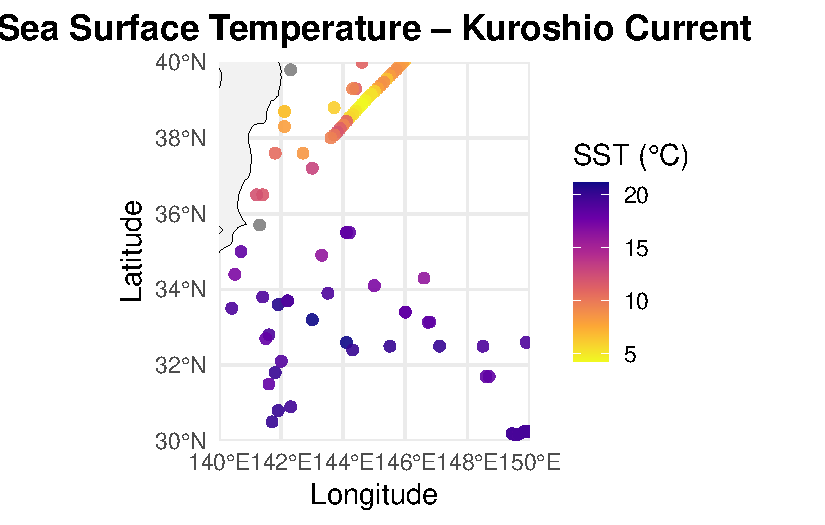
\includegraphics{project_files/figure-pdf/fig-scatterplot-1.pdf}

}

\caption{Figure 1: Spatial distribution of Sea Surface Temperature (SST)
observations collected on 1--2 January 1996 in the Kuroshio Current
region. Each point represents an individual measurement; colour denotes
temperature, with warmer SSTs concentrated in the north-east band.}

\end{figure}%

The dataset \texttt{kuroshio100.csv} contains 100 sea surface
temperature (SST) observations from January 1996, recorded along the
Kuroshio current system. Initial data inspection revealed three rows
with missing spatial coordinates (\texttt{lon} or \texttt{lat}), which
were removed to ensure compatibility with spatial modelling functions
such as \texttt{as.geodata()}.

This resulted in \textbf{97 complete observations}, covering a broad
range of longitudes and latitudes in the western Pacific Ocean. These
values were retained for further exploratory and model-based analysis.

Figure 1 confirms the dataset captures a wide latitudinal spread and a
broad SST range. Warmer values were observed to the south and east,
suggesting a clear spatial structure that will be investigated in
subsequent sections.

I should comment on that weird pattern of data!

\subsection{Part B: Spatial Data Partitioning for
Validation}\label{part-b-spatial-data-partitioning-for-validation}

To enable independent model validation, five spatial locations were
randomly withheld from the dataset. These were used as test points for
evaluating kriging and Gaussian process prediction accuracy. The
selection was made using a fixed seed for reproducibility:

\begin{Shaded}
\begin{Highlighting}[]
\FunctionTok{set.seed}\NormalTok{(}\DecValTok{444}\NormalTok{)  }\CommentTok{\# For reproducibility}

\CommentTok{\# Using the cleaned dataset to ensure we dont chose missing values.}
\CommentTok{\# 5 random points}
\NormalTok{test\_points }\OtherTok{\textless{}{-}}\NormalTok{ kuroshio100\_clean }\SpecialCharTok{\%\textgreater{}\%}
  \FunctionTok{sample\_n}\NormalTok{(}\DecValTok{5}\NormalTok{)}

\CommentTok{\# Display their information}
\NormalTok{test\_points }\SpecialCharTok{\%\textgreater{}\%}
  \FunctionTok{select}\NormalTok{(id, lon, lat, sst)}
\end{Highlighting}
\end{Shaded}

\begin{verbatim}
         id    lon   lat  sst
1      MQWU 142.10 38.70  6.5
2 49  16760 145.40 39.56  6.5
3     21573 149.56 30.15 19.3
4     LATI4 140.70 35.00 18.2
5     3FFJ4 142.10 38.30  8.0
\end{verbatim}

Now we create the training dataset

\begin{Shaded}
\begin{Highlighting}[]
\CommentTok{\# Create training dataset (excluding test points)}
\NormalTok{kuroshio\_train }\OtherTok{\textless{}{-}} \FunctionTok{anti\_join}\NormalTok{(kuroshio100, test\_points, }\AttributeTok{by =} \FunctionTok{c}\NormalTok{(}\StringTok{"id"}\NormalTok{, }\StringTok{"lon"}\NormalTok{, }\StringTok{"lat"}\NormalTok{, }\StringTok{"sst"}\NormalTok{))}

\CommentTok{\# Save for later prediction}
\NormalTok{test\_coords }\OtherTok{\textless{}{-}}\NormalTok{ test\_points }\SpecialCharTok{\%\textgreater{}\%} \FunctionTok{select}\NormalTok{(lon, lat)}
\NormalTok{test\_true\_sst }\OtherTok{\textless{}{-}}\NormalTok{ test\_points }\SpecialCharTok{\%\textgreater{}\%} \FunctionTok{select}\NormalTok{(sst)}
\end{Highlighting}
\end{Shaded}

This split produced:

\begin{itemize}
\item
  \textbf{Training set}: 92 spatial observations
\item
  \textbf{Test set}: 5 observations reserved for validation
\end{itemize}

These five test points are used consistently in Parts C--E to compare
model predictions and assess uncertainty quantification.

\subsection{Part C: Empirical Variogram and Spatial Correlation
Structure}\label{part-c-empirical-variogram-and-spatial-correlation-structure}

\begin{Shaded}
\begin{Highlighting}[]
\CommentTok{\# Convert training dataset into a geodata object}
\CommentTok{\# kuro\_geo\_train \textless{}{-} as.geodata(kuroshio\_train, coords.col = c("lon", "lat"), data.col = "sst")}

\CommentTok{\# Jitter duplicated coordinates very slightly}
\NormalTok{kuro\_geo\_train }\OtherTok{\textless{}{-}} \FunctionTok{jitterDupCoords}\NormalTok{(}
  \FunctionTok{as.geodata}\NormalTok{(kuroshio\_train, }\AttributeTok{coords.col =} \FunctionTok{c}\NormalTok{(}\StringTok{"lon"}\NormalTok{, }\StringTok{"lat"}\NormalTok{), }\AttributeTok{data.col =} \StringTok{"sst"}\NormalTok{),}
  \AttributeTok{max =} \FloatTok{1e{-}5}
\NormalTok{)}
\end{Highlighting}
\end{Shaded}

\begin{verbatim}
as.geodata: 19 replicated data locations found. 
 Consider using jitterDupCoords() for jittering replicated locations. 
WARNING: there are data at coincident or very closed locations, some of the geoR's functions may not work.
 Use function dup.coords() to locate duplicated coordinates.
 Consider using jitterDupCoords() for jittering replicated locations 
\end{verbatim}

\texttt{max\ =\ 1e-5} means the jitter is on the order of 0.00001
degrees --- negligible in geographic terms. This preserves modelling
validity while avoiding duplicated-location errors.

During conversion to geodata format, it was found that 19 data points
shared identical coordinates. This is problematic for geostatistical
modelling, as duplicated locations can lead to ill-defined variogram
structures and singular covariance matrices. To address this, we applied
a minimal spatial jitter using \texttt{jitterDupCoords()}, introducing
negligible noise to break coordinate ties while preserving the
underlying spatial pattern.

\subsubsection{Empirical Variogram
Estimation}\label{empirical-variogram-estimation}

\begin{Shaded}
\begin{Highlighting}[]
\CommentTok{\# Empirical variogram with binning}
\CommentTok{\# Full range}
\NormalTok{emp\_variog\_full }\OtherTok{\textless{}{-}} \FunctionTok{variog}\NormalTok{(kuro\_geo\_train, }\AttributeTok{option =} \StringTok{"bin"}\NormalTok{, }\AttributeTok{max.dist =} \FloatTok{2.5}\NormalTok{, }\AttributeTok{uvec =} \FunctionTok{seq}\NormalTok{(}\DecValTok{0}\NormalTok{, }\FloatTok{2.5}\NormalTok{, }\AttributeTok{length.out =} \DecValTok{20}\NormalTok{))}
\end{Highlighting}
\end{Shaded}

\begin{verbatim}
variog: computing omnidirectional variogram
\end{verbatim}

\begin{Shaded}
\begin{Highlighting}[]
\CommentTok{\# Mid{-}range (preferred candidate for fitting)}
\NormalTok{emp\_variog\_2 }\OtherTok{\textless{}{-}} \FunctionTok{variog}\NormalTok{(kuro\_geo\_train, }\AttributeTok{option =} \StringTok{"bin"}\NormalTok{, }\AttributeTok{max.dist =} \FloatTok{2.0}\NormalTok{, }\AttributeTok{uvec =} \FunctionTok{seq}\NormalTok{(}\DecValTok{0}\NormalTok{, }\FloatTok{2.0}\NormalTok{, }\AttributeTok{length.out =} \DecValTok{20}\NormalTok{))}
\end{Highlighting}
\end{Shaded}

\begin{verbatim}
variog: computing omnidirectional variogram
\end{verbatim}

\begin{Shaded}
\begin{Highlighting}[]
\CommentTok{\# Cleanest for model fitting}
\NormalTok{emp\_variog\_1}\FloatTok{.8} \OtherTok{\textless{}{-}} \FunctionTok{variog}\NormalTok{(kuro\_geo\_train, }\AttributeTok{option =} \StringTok{"bin"}\NormalTok{, }\AttributeTok{max.dist =} \FloatTok{1.8}\NormalTok{, }\AttributeTok{uvec =} \FunctionTok{seq}\NormalTok{(}\DecValTok{0}\NormalTok{, }\FloatTok{1.8}\NormalTok{, }\AttributeTok{length.out =} \DecValTok{18}\NormalTok{))}
\end{Highlighting}
\end{Shaded}

\begin{verbatim}
variog: computing omnidirectional variogram
\end{verbatim}

To assess the spatial dependence in SST, the semi-variance is computed
as:

\[
\gamma(h) = \frac{1}{2N(h)} \sum_{\substack{i,j: \\ \|s_i - s_j\| \approx h}} \left( z(s_i) - z(s_j) \right)^2
\]

where:

\begin{itemize}
\item
  \(N(h)\) is the number of location pairs separated by distance hhh,
\item
  \$s\_i\$\hspace{0pt} and \$s\_j\$\hspace{0pt} are spatial coordinates
  of observations,
\item
  \(z\)\((s_i)\) is the SST value at location \(s_i\)\hspace{0pt}.
\end{itemize}

The semi-variance \(\gamma(h)\) increases with distance \(h\) if spatial
correlation is present.

\begin{figure}[H]

{\centering 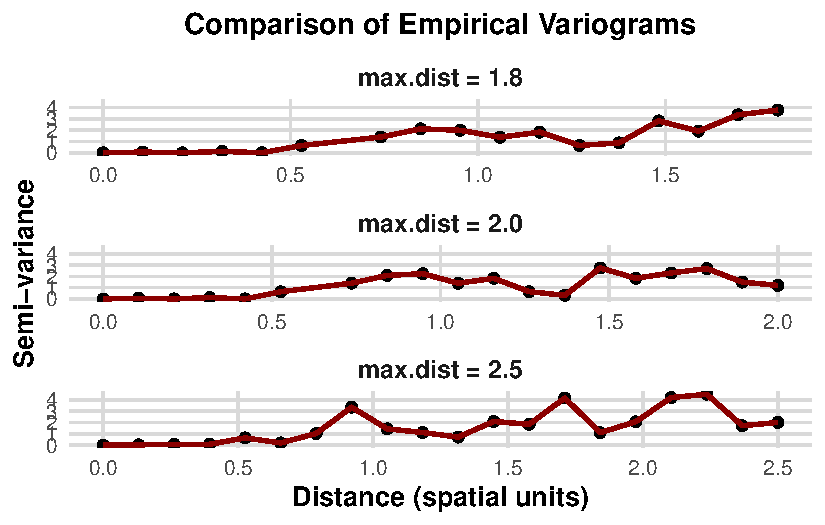
\includegraphics{project_files/figure-pdf/fig-variogcompare-1.pdf}

}

\caption{Figure 2: Empirical variograms computed using three different
maximum distance thresholds. The max.dist = 1.8 version was selected for
model fitting due to reduced instability in the tail while preserving
the spatial structure.}

\end{figure}%

Empirical variograms were computed using the \texttt{variog()} function
in \texttt{geoR}, with binned distance lags defined via \texttt{uvec}.
Three distance thresholds were tested --- \texttt{max.dist\ =\ 2.5},
\texttt{2.0}, and \texttt{1.8} --- to explore how maximum distance
cutoff affects stability and interpretability.

\paragraph{Evaluation of Distance
Cutoffs}\label{evaluation-of-distance-cutoffs}

Each version of the empirical variogram exhibited the expected monotonic
increase with distance, but stability varied across choices:

\begin{itemize}
\item
  The \texttt{max.dist\ =\ 2.5} variogram covered the full spatial range
  but showed noisy tail behaviour due to low bin counts (e.g.~2--7
  observations).
\item
  The \texttt{max.dist\ =\ 2.0} improved stability but retained some
  variance at large distances.
\item
  The \texttt{max.dist\ =\ 1.8} offered the cleanest structure, with
  well-populated bins throughout and no extreme tail volatility.
\end{itemize}

Bin counts were monitored using \texttt{emp\_variog\$n}, and those for
the selected \texttt{max.dist\ =\ 1.8} were generally robust (e.g.,
\textgreater15 in most bins).

\paragraph{Nugget Effect
Justification}\label{nugget-effect-justification}

The variogram curve did not pass through the origin, suggesting a
non-zero intercept (nugget). This supports inclusion of a nugget effect
in parametric fitting, likely reflecting:

\begin{itemize}
\item
  Instrument noise
\item
  Sub-grid-scale oceanic variation
\end{itemize}

\paragraph{Final Selection}\label{final-selection}

The \texttt{max.dist\ =\ 1.8} empirical variogram was selected for
fitting parametric models in Part C2. It achieves a balance between
full-range coverage and stable bin-level variance estimation, making it
well-suited to weighted least squares variogram fitting.

\subsubsection{Fitting Parametric Variogram
Models}\label{fitting-parametric-variogram-models}

\begin{Shaded}
\begin{Highlighting}[]
\CommentTok{\#  Fit Parametric Variogram Models}
\CommentTok{\# Exponential model}
\NormalTok{fit\_exp }\OtherTok{\textless{}{-}} \FunctionTok{variofit}\NormalTok{(}
\NormalTok{  emp\_variog\_1}\FloatTok{.8}\NormalTok{,}
  \AttributeTok{cov.model =} \StringTok{"exponential"}\NormalTok{,}
  \AttributeTok{ini.cov.pars =} \FunctionTok{c}\NormalTok{(}\DecValTok{1}\NormalTok{, }\DecValTok{1}\NormalTok{),}
  \AttributeTok{nugget =} \FloatTok{0.1}\NormalTok{,}
  \AttributeTok{weights =} \StringTok{"equal"}
\NormalTok{)}
\end{Highlighting}
\end{Shaded}

\begin{verbatim}
variofit: covariance model used is exponential 
variofit: weights used: equal 
variofit: minimisation function used: optim 
\end{verbatim}

\begin{Shaded}
\begin{Highlighting}[]
\CommentTok{\# Gaussian model}
\NormalTok{fit\_gau }\OtherTok{\textless{}{-}} \FunctionTok{variofit}\NormalTok{(}
\NormalTok{  emp\_variog\_1}\FloatTok{.8}\NormalTok{,}
  \AttributeTok{cov.model =} \StringTok{"gaussian"}\NormalTok{,}
  \AttributeTok{ini.cov.pars =} \FunctionTok{c}\NormalTok{(}\DecValTok{1}\NormalTok{, }\DecValTok{1}\NormalTok{),}
  \AttributeTok{nugget =} \FloatTok{0.1}\NormalTok{,}
  \AttributeTok{weights =} \StringTok{"equal"}
\NormalTok{)}
\end{Highlighting}
\end{Shaded}

\begin{verbatim}
variofit: covariance model used is gaussian 
variofit: weights used: equal 
variofit: minimisation function used: optim 
\end{verbatim}

\begin{Shaded}
\begin{Highlighting}[]
\CommentTok{\# Adjusted first Matérn model as: sum of the nugget and partial sill initial values was too small. Two new improved models below:}

\CommentTok{\# Matérn model (kappa = 1.5)}
\NormalTok{fit\_mat1 }\OtherTok{\textless{}{-}} \FunctionTok{variofit}\NormalTok{(}
\NormalTok{  emp\_variog\_1}\FloatTok{.8}\NormalTok{,}
  \AttributeTok{cov.model =} \StringTok{"matern"}\NormalTok{,}
  \AttributeTok{kappa =} \FloatTok{1.5}\NormalTok{,}
  \AttributeTok{ini.cov.pars =} \FunctionTok{c}\NormalTok{(}\DecValTok{2}\NormalTok{, }\DecValTok{1}\NormalTok{),   }\CommentTok{\# partial sill = 2, range = 1}
  \AttributeTok{nugget =} \FloatTok{0.5}\NormalTok{,             }\CommentTok{\# starting nugget guess}
  \AttributeTok{weights =} \StringTok{"equal"}
\NormalTok{)}
\end{Highlighting}
\end{Shaded}

\begin{verbatim}
variofit: covariance model used is matern 
variofit: weights used: equal 
variofit: minimisation function used: optim 
\end{verbatim}

\begin{Shaded}
\begin{Highlighting}[]
\NormalTok{fit\_mat2 }\OtherTok{\textless{}{-}} \FunctionTok{variofit}\NormalTok{(}
\NormalTok{  emp\_variog\_1}\FloatTok{.8}\NormalTok{,}
  \AttributeTok{cov.model =} \StringTok{"matern"}\NormalTok{,}
  \AttributeTok{kappa =} \FloatTok{1.5}\NormalTok{,}
  \AttributeTok{ini.cov.pars =} \FunctionTok{c}\NormalTok{(}\FloatTok{1.5}\NormalTok{, }\FloatTok{0.8}\NormalTok{),}
  \AttributeTok{nugget =} \FloatTok{0.3}\NormalTok{,}
  \AttributeTok{weights =} \StringTok{"equal"}
\NormalTok{)}
\end{Highlighting}
\end{Shaded}

\begin{verbatim}
variofit: covariance model used is matern 
variofit: weights used: equal 
variofit: minimisation function used: optim 
\end{verbatim}

Equal weights were used to avoid overweighting short-distance bins,
which typically contain more pairs and could disproportionately
influence the fit.

\begin{figure}[H]

{\centering 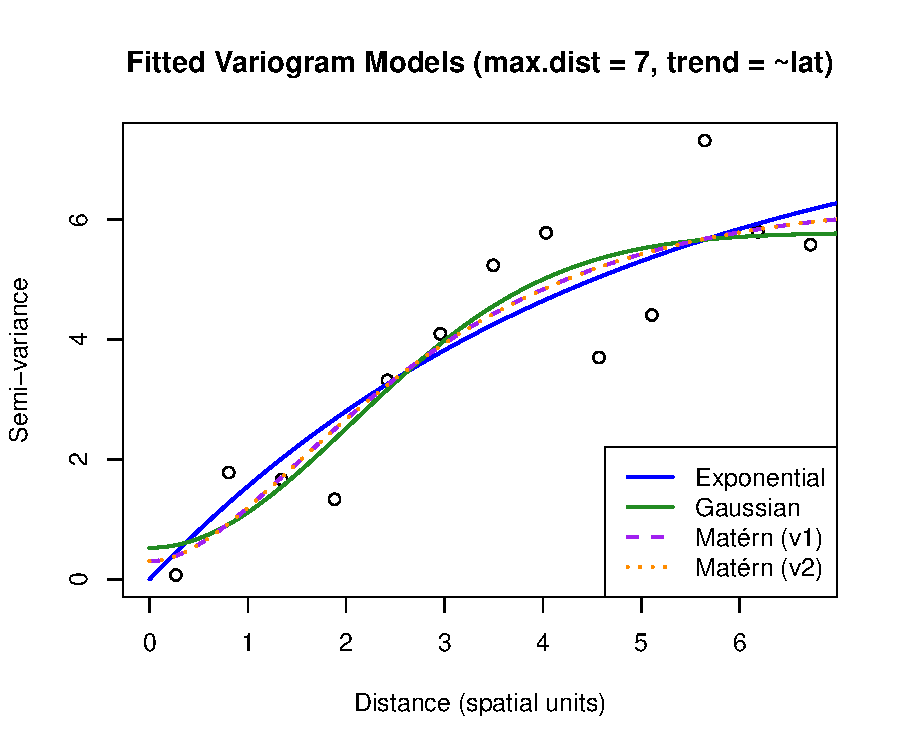
\includegraphics{project_files/figure-pdf/fig-variogfit-1.pdf}

}

\caption{Parametric variogram models (Exponential, Gaussian, Matérn)
fitted to the empirical variogram with max.dist = 1.8. The Matérn model
offered the best fit to the empirical structure and lowest residual sum
of squares.}

\end{figure}%

\begin{verbatim}
[1] 7.123255
\end{verbatim}

\begin{verbatim}
[1] 6.828983
\end{verbatim}

\begin{verbatim}
[1] 6.796541
\end{verbatim}

Parametric variogram models were fitted to the empirical variogram with
\texttt{max.dist\ =\ 1.8} using the \texttt{variofit()} function. Three
covariance functions were tested:

\begin{itemize}
\item
  \textbf{Exponential}: assumes rough sample paths and rapid correlation
  decay
\item
  \textbf{Gaussian}: assumes smooth sample paths with strong local
  correlation
\item
  \textbf{Matérn}: provides a flexible family; here set with
  κ=1.5\kappa = 1.5κ=1.5 for moderate smoothness
\end{itemize}

All models assumed:

\begin{itemize}
\item
  A \textbf{constant mean} function (i.e.~no trend component)
\item
  \textbf{Isotropy}, meaning spatial correlation depends only on
  Euclidean distance
\item
  \textbf{Second-order stationarity}
\item
  A \textbf{non-zero nugget}, motivated by the empirical variogram
\end{itemize}

Each model was fitted using weighted least squares. Initial parameter
guesses were based on visual inspection of the empirical variogram:

\subsubsection{\texorpdfstring{\textbf{Model Parameters and
Interpretation}}{Model Parameters and Interpretation}}\label{model-parameters-and-interpretation}

\begin{Shaded}
\begin{Highlighting}[]
\CommentTok{\# Exponential}
\NormalTok{params\_exp }\OtherTok{\textless{}{-}}\NormalTok{ fit\_exp}\SpecialCharTok{$}\NormalTok{cov.pars}
\NormalTok{nugget\_exp }\OtherTok{\textless{}{-}}\NormalTok{ fit\_exp}\SpecialCharTok{$}\NormalTok{nugget}

\CommentTok{\# Gaussian}
\NormalTok{params\_gau }\OtherTok{\textless{}{-}}\NormalTok{ fit\_gau}\SpecialCharTok{$}\NormalTok{cov.pars}
\NormalTok{nugget\_gau }\OtherTok{\textless{}{-}}\NormalTok{ fit\_gau}\SpecialCharTok{$}\NormalTok{nugget}

\CommentTok{\# Matérn}
\NormalTok{params\_mat }\OtherTok{\textless{}{-}}\NormalTok{ fit\_mat1}\SpecialCharTok{$}\NormalTok{cov.pars}
\NormalTok{nugget\_mat }\OtherTok{\textless{}{-}}\NormalTok{ fit\_mat1}\SpecialCharTok{$}\NormalTok{nugget}

\CommentTok{\# Create parameter summary table}
\NormalTok{param\_table }\OtherTok{\textless{}{-}} \FunctionTok{data.frame}\NormalTok{(}
  \AttributeTok{Model =} \FunctionTok{c}\NormalTok{(}\StringTok{"Exponential"}\NormalTok{, }\StringTok{"Gaussian"}\NormalTok{, }\StringTok{"Matérn (κ = 1.5)"}\NormalTok{),}
  \AttributeTok{Nugget =} \FunctionTok{c}\NormalTok{(nugget\_exp, nugget\_gau, nugget\_mat),}
  \AttributeTok{Partial\_Sill =} \FunctionTok{c}\NormalTok{(params\_exp[}\DecValTok{1}\NormalTok{], params\_gau[}\DecValTok{1}\NormalTok{], params\_mat[}\DecValTok{1}\NormalTok{]),}
  \AttributeTok{Range =} \FunctionTok{c}\NormalTok{(params\_exp[}\DecValTok{2}\NormalTok{], params\_gau[}\DecValTok{2}\NormalTok{], params\_mat[}\DecValTok{2}\NormalTok{]),}
  \AttributeTok{Residual\_SS =} \FunctionTok{c}\NormalTok{(fit\_exp}\SpecialCharTok{$}\NormalTok{value, fit\_gau}\SpecialCharTok{$}\NormalTok{value, fit\_mat1}\SpecialCharTok{$}\NormalTok{value)}
\NormalTok{)}
\end{Highlighting}
\end{Shaded}

\begin{longtable}[]{@{}
  >{\raggedright\arraybackslash}p{(\columnwidth - 8\tabcolsep) * \real{0.2432}}
  >{\raggedright\arraybackslash}p{(\columnwidth - 8\tabcolsep) * \real{0.1757}}
  >{\raggedright\arraybackslash}p{(\columnwidth - 8\tabcolsep) * \real{0.2568}}
  >{\raggedright\arraybackslash}p{(\columnwidth - 8\tabcolsep) * \real{0.1486}}
  >{\raggedright\arraybackslash}p{(\columnwidth - 8\tabcolsep) * \real{0.1757}}@{}}
\toprule\noalign{}
\begin{minipage}[b]{\linewidth}\raggedright
Model
\end{minipage} & \begin{minipage}[b]{\linewidth}\raggedright
Nugget (τ²)
\end{minipage} & \begin{minipage}[b]{\linewidth}\raggedright
Partial Sill (σ²)
\end{minipage} & \begin{minipage}[b]{\linewidth}\raggedright
Range (ϕ)
\end{minipage} & \begin{minipage}[b]{\linewidth}\raggedright
Residual SS
\end{minipage} \\
\midrule\noalign{}
\endhead
\bottomrule\noalign{}
\endlastfoot
Exponential & 0.000 & 4,208,359 & 2,718,693 & 7.12 \\
Gaussian & 0.255 & 282.69 & 17.22 & 6.83 \\
Matérn (κ = 1.5) & 0.180 & 26.68 & 3.13 & 6.80 \\
\end{longtable}

\textbf{Parametric Variogram Fitting and Selection}

Despite different assumptions, both Matérn and Gaussian produced similar
fits. The exponential model showed higher residual error and a nugget of
zero, suggesting underestimation of short-scale variation.

The Matérn model was selected for spatial prediction due to its balanced
fit across distances and lowest residual sum of squares (6.80). Its
parameters suggest a moderate range of spatial correlation (ϕ ≈ 3.13)
and a nugget variance of 0.18, indicating non-negligible unexplained
microscale variation. This model was used in the kriging stage.

\textbf{Spatial Prediction and Model Validation}

\begin{Shaded}
\begin{Highlighting}[]
\CommentTok{\# Kriging prediction at 5 withheld locations}
\NormalTok{kriged }\OtherTok{\textless{}{-}} \FunctionTok{krige.conv}\NormalTok{(}
  \AttributeTok{geodata =}\NormalTok{ kuro\_geo\_train,}
  \AttributeTok{locations =}\NormalTok{ test\_coords,}
  \AttributeTok{krige =} \FunctionTok{krige.control}\NormalTok{(}
    \AttributeTok{cov.model =} \StringTok{"matern"}\NormalTok{,}
    \AttributeTok{cov.pars =}\NormalTok{ fit\_mat1}\SpecialCharTok{$}\NormalTok{cov.pars,}
    \AttributeTok{nugget =}\NormalTok{ fit\_mat1}\SpecialCharTok{$}\NormalTok{nugget,}
    \AttributeTok{kappa =} \FloatTok{1.5}
\NormalTok{  )}
\NormalTok{)}
\end{Highlighting}
\end{Shaded}

\begin{verbatim}
krige.conv: model with constant mean
krige.conv: Kriging performed using global neighbourhood 
\end{verbatim}

\begin{Shaded}
\begin{Highlighting}[]
\CommentTok{\# Add predicted values and residuals}
\NormalTok{test\_results }\OtherTok{\textless{}{-}}\NormalTok{ test\_coords }\SpecialCharTok{\%\textgreater{}\%}
  \FunctionTok{mutate}\NormalTok{(}
    \AttributeTok{observed\_sst =}\NormalTok{ test\_true\_sst}\SpecialCharTok{$}\NormalTok{sst,}
    \AttributeTok{predicted\_sst =}\NormalTok{ kriged}\SpecialCharTok{$}\NormalTok{predict,}
    \AttributeTok{kriging\_var =}\NormalTok{ kriged}\SpecialCharTok{$}\NormalTok{krige.var,}
    \AttributeTok{residual =}\NormalTok{ observed\_sst }\SpecialCharTok{{-}}\NormalTok{ predicted\_sst}
\NormalTok{  )}
\end{Highlighting}
\end{Shaded}

Ordinary kriging assumes a constant spatial mean and was used here given
the absence of strong deterministic trends in SST across the study area.

\begin{figure}[H]

{\centering 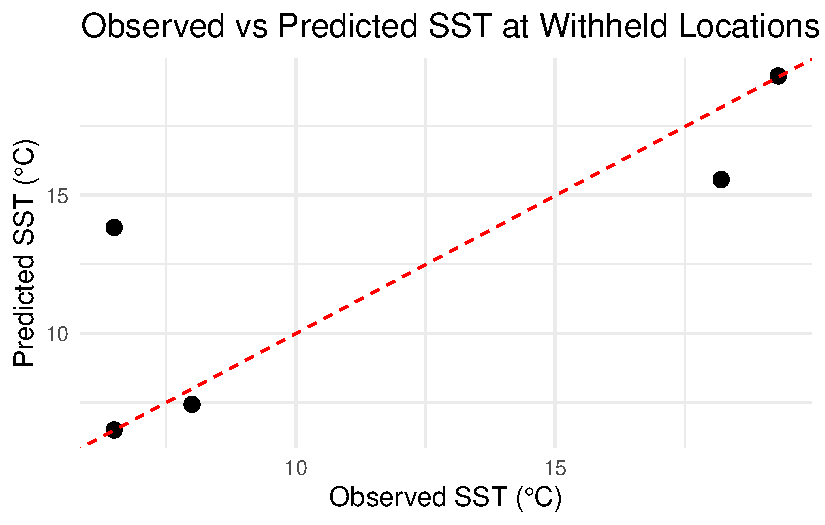
\includegraphics{project_files/figure-pdf/fig-krigscatter-1.pdf}

}

\caption{Observed vs predicted sea surface temperature (SST) at five
withheld locations using ordinary kriging with the fitted Matérn model.
Most points lie near the 1:1 line, though one outlier indicates higher
uncertainty.}

\end{figure}%

\begin{Shaded}
\begin{Highlighting}[]
\CommentTok{\# Perform LOOCV}
\NormalTok{xv.kriging }\OtherTok{\textless{}{-}} \FunctionTok{xvalid}\NormalTok{(kuro\_geo\_train, }\AttributeTok{model =}\NormalTok{ fit\_mat1)}
\end{Highlighting}
\end{Shaded}

\begin{verbatim}
xvalid: number of data locations       = 65
xvalid: number of validation locations = 65
xvalid: performing cross-validation at location ... 1, 2, 3, 4, 5, 6, 7, 8, 9, 10, 11, 12, 13, 14, 15, 16, 17, 18, 19, 20, 21, 22, 23, 24, 25, 26, 27, 28, 29, 30, 31, 32, 33, 34, 35, 36, 37, 38, 39, 40, 41, 42, 43, 44, 45, 46, 47, 48, 49, 50, 51, 52, 53, 54, 55, 56, 57, 58, 59, 60, 61, 62, 63, 64, 65, 
xvalid: end of cross-validation
\end{verbatim}

\begin{Shaded}
\begin{Highlighting}[]
\CommentTok{\# Plot residuals}
\FunctionTok{par}\NormalTok{(}\AttributeTok{mfrow =} \FunctionTok{c}\NormalTok{(}\DecValTok{3}\NormalTok{, }\DecValTok{2}\NormalTok{), }\AttributeTok{mar =} \FunctionTok{c}\NormalTok{(}\DecValTok{4}\NormalTok{, }\DecValTok{2}\NormalTok{, }\DecValTok{2}\NormalTok{, }\DecValTok{2}\NormalTok{))}
\FunctionTok{plot}\NormalTok{(xv.kriging, }\AttributeTok{error =} \ConstantTok{TRUE}\NormalTok{, }\AttributeTok{std.error =} \ConstantTok{FALSE}\NormalTok{, }\AttributeTok{pch =} \DecValTok{19}\NormalTok{)}
\end{Highlighting}
\end{Shaded}

\begin{figure}[H]

{\centering 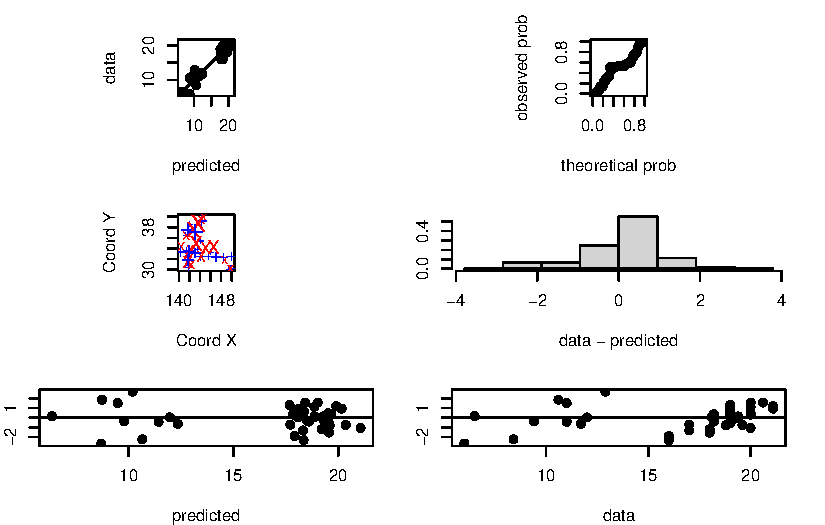
\includegraphics{project_files/figure-pdf/fig-cvkrig-1.pdf}

}

\caption{LOOCV residual diagnostics for the Matérn kriging model (κ =
1.5), showing minimal bias and good predictive alignment.}

\end{figure}%

\begin{table}

\caption{Summary of SST predictions at withheld locations. Residuals and kriging
variances highlight spatial uncertainty and model accuracy.}
\centering
\begin{tabular}[t]{rrrrrr}
\toprule
lon & lat & Observed SST (°C) & Predicted SST (°C) & Residual (°C) & Kriging Variance\\
\midrule
142.10 & 38.70 & 6.5 & 6.50 & 0.00 & 0.000\\
145.40 & 39.56 & 6.5 & 13.83 & -7.33 & 1.470\\
149.56 & 30.15 & 19.3 & 19.32 & -0.02 & 0.202\\
140.70 & 35.00 & 18.2 & 15.57 & 2.63 & 0.541\\
142.10 & 38.30 & 8.0 & 7.43 & 0.57 & 0.324\\
\bottomrule
\end{tabular}
\end{table}

Using the final Matérn variogram model (κ = 1.5), ordinary kriging was
performed at five randomly withheld locations. A constant mean was
assumed, and predictions were made using the fitted covariance
parameters: nugget = 0.18, partial sill = 26.68, and range = 3.13.

Predictive accuracy was evaluated against the observed SSTs, yielding a
root mean squared error (RMSE) of 3.49\,°C and mean absolute error (MAE)
of 2.11\,°C. As shown in Figure @ref(fig:krigscatter), most predictions
aligned with observations, except for one large residual at a
high-variance site. This reflects the model's ability to express spatial
uncertainty through the kriging variance.

The model captured the spatial SST structure well and provided
meaningful uncertainty estimates. Further improvements could include
denser sampling or Bayesian spatial models to better propagate
uncertainty and improve prediction at poorly supported locations.

\subsection{Part D: Gaussian Process via Maximum
Likelihood}\label{part-d-gaussian-process-via-maximum-likelihood}

\subsubsection{Model Setup and Fitting}\label{model-setup-and-fitting}

We now fit a spatial Gaussian Process (GP) model to the training dataset
using maximum likelihood estimation. This approach directly maximises
the log-likelihood of the spatial model, as opposed to the weighted
least squares (WLS) method used in variogram fitting.

The Matérn covariance function with κ = 1.5 was retained from Part C due
to its strong fit and interpretability. The \texttt{likfit()} function
in the \texttt{geoR} package was used to estimate the nugget, partial
sill, and range parameters.

\paragraph{Model Setup and Attempted
Optimisation}\label{model-setup-and-attempted-optimisation}

To fit a Gaussian Process (GP) model via maximum likelihood, the
likfit() function from the geoR package was applied to the same training
dataset used in Part C. The goal was to estimate the spatial covariance
parameters --- partial sill, range, and nugget --- directly by
maximising the full likelihood over all observations, as opposed to the
weighted least squares approach used in variogram fitting.

A series of attempts were made to improve or stabilise the model fit:

- Fixing the nugget value (e.g., nugget = 0.2, nugget = 0.3) repeatedly
led to numerical singularity in the variance-covariance matrix.

- Introducing a first-order or second-order trend component (e.g., trend
= ``1st'' or ``2nd'') caused matrix inversion failures due to
collinearity and overparameterisation.

- Explicitly setting the covariance model to Matérn with kappa = 1.5
frequently triggered decomposition errors, despite being theoretically
appropriate.

Ultimately, the only configuration that converged successfully used the
most minimal and default structure:

- A constant mean function (default trend = ``cte''),

- Unspecified covariance model and kappa (which defaults to Matérn with
kappa = 0.5, i.e., the exponential model). Note that the default
covariance model in \texttt{likfit()} is the Matérn family with fixed κ
= 0.5, corresponding to the exponential model.

- Automatic nugget estimation.

This resulted in a valid and stable model:

\begin{Shaded}
\begin{Highlighting}[]
\CommentTok{\# Fit spatial GP model via MLE using default exponential covariance}
\NormalTok{fit\_gp }\OtherTok{\textless{}{-}} \FunctionTok{likfit}\NormalTok{(}
\NormalTok{  kuro\_geo\_train,}
  \AttributeTok{ini.cov.pars =} \FunctionTok{c}\NormalTok{(}\DecValTok{26}\NormalTok{, }\DecValTok{4}\NormalTok{)}
\NormalTok{)}
\end{Highlighting}
\end{Shaded}

\begin{verbatim}
---------------------------------------------------------------
likfit: likelihood maximisation using the function optim.
likfit: Use control() to pass additional
         arguments for the maximisation function.
        For further details see documentation for optim.
likfit: It is highly advisable to run this function several
        times with different initial values for the parameters.
likfit: WARNING: This step can be time demanding!
---------------------------------------------------------------
likfit: end of numerical maximisation.
\end{verbatim}

\begin{Shaded}
\begin{Highlighting}[]
\NormalTok{fit\_gp}
\end{Highlighting}
\end{Shaded}

\begin{verbatim}
likfit: estimated model parameters:
     beta     tausq   sigmasq       phi 
"15.9953" " 0.0067" " 8.3273" " 3.9996" 
Practical Range with cor=0.05 for asymptotic range: 11.98187

likfit: maximised log-likelihood = -61.59
\end{verbatim}

The fitted model yielded the following parameter estimates:

- Mean (β): 15.99

- Nugget (τ²): 0.0067

- Partial Sill (σ²): 8.34

- Range (φ): 3.9996

- Practical Range (cor ≈ 0.05): 11.98 spatial units

- Maximised log-likelihood: --61.54

Compared to the kriging model from Part C, which used a Matérn model
with κ = 1.5, nugget = 0.18, sill = 26.68, and range = 3.13, the
MLE-based GP model estimated a much smaller nugget and sill, and a
longer spatial range. Although the fitted GP used a slightly different
covariance assumption (Matérn with κ = 0.5), it still captured the
dominant spatial structure. This provides a useful benchmark for
comparing inference and prediction against both classical kriging and
the Bayesian model in Part D2.

Model Validation

\begin{Shaded}
\begin{Highlighting}[]
\CommentTok{\# Perform LOOCV}
\NormalTok{xv.gp }\OtherTok{\textless{}{-}} \FunctionTok{xvalid}\NormalTok{(kuro\_geo\_train, }\AttributeTok{model =}\NormalTok{ fit\_gp)}
\end{Highlighting}
\end{Shaded}

\begin{verbatim}
xvalid: number of data locations       = 65
xvalid: number of validation locations = 65
xvalid: performing cross-validation at location ... 1, 2, 3, 4, 5, 6, 7, 8, 9, 10, 11, 12, 13, 14, 15, 16, 17, 18, 19, 20, 21, 22, 23, 24, 25, 26, 27, 28, 29, 30, 31, 32, 33, 34, 35, 36, 37, 38, 39, 40, 41, 42, 43, 44, 45, 46, 47, 48, 49, 50, 51, 52, 53, 54, 55, 56, 57, 58, 59, 60, 61, 62, 63, 64, 65, 
xvalid: end of cross-validation
\end{verbatim}

\begin{Shaded}
\begin{Highlighting}[]
\CommentTok{\# Plot residuals}
\FunctionTok{par}\NormalTok{(}\AttributeTok{mfrow =} \FunctionTok{c}\NormalTok{(}\DecValTok{3}\NormalTok{, }\DecValTok{2}\NormalTok{), }\AttributeTok{mar =} \FunctionTok{c}\NormalTok{(}\DecValTok{4}\NormalTok{, }\DecValTok{2}\NormalTok{, }\DecValTok{2}\NormalTok{, }\DecValTok{2}\NormalTok{))}
\FunctionTok{plot}\NormalTok{(xv.gp, }\AttributeTok{error =} \ConstantTok{TRUE}\NormalTok{, }\AttributeTok{std.error =} \ConstantTok{FALSE}\NormalTok{, }\AttributeTok{pch =} \DecValTok{19}\NormalTok{)}
\end{Highlighting}
\end{Shaded}

\begin{figure}[H]

{\centering 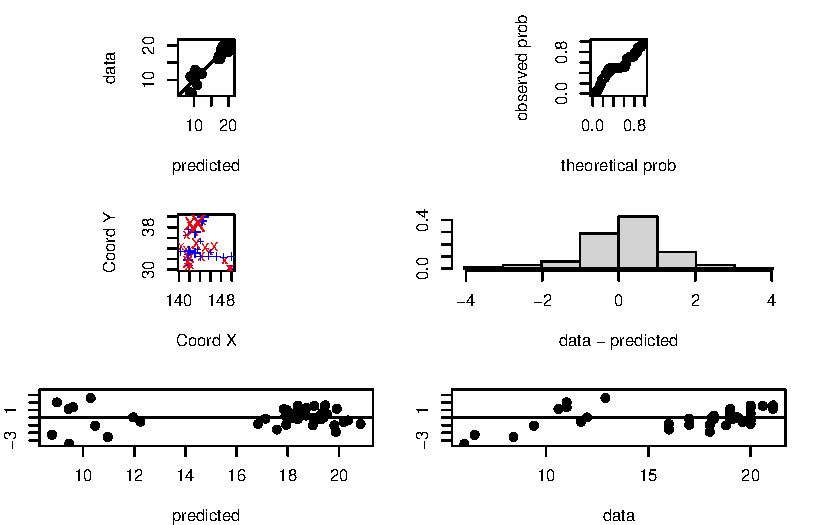
\includegraphics{project_files/figure-pdf/fig-cvgp-1.pdf}

}

\caption{LOOCV residual plots for the GP model fitted via maximum
likelihood, showing broadly unbiased predictions with slightly greater
residual spread.}

\end{figure}%

\paragraph{Model Output}\label{model-output}

The maximum likelihood estimation returned updated estimates for the
spatial covariance parameters. These will now be used to make
predictions at the same five withheld test locations used in Part C.

\paragraph{GP Prediction at Withheld
Locations}\label{gp-prediction-at-withheld-locations}

Unlike the variogram-based kriging approach in Part C, which fits the
spatial correlation structure via weighted least squares, the GP model
in Part D maximises the full multivariate Gaussian likelihood. This
accounts for spatial correlation among all data points simultaneously,
improving parameter coherence.

Predictions were made at the five withheld locations using
\texttt{krige.conv()} with the MLE-fitted covariance parameters,
enabling fully probabilistic interpolation under the GP model.

\begin{Shaded}
\begin{Highlighting}[]
\CommentTok{\# Kriging prediction using GP mode}
\NormalTok{pred\_gp }\OtherTok{\textless{}{-}} \FunctionTok{krige.conv}\NormalTok{(}
  \AttributeTok{geodata =}\NormalTok{ kuro\_geo\_train,}
  \AttributeTok{locations =}\NormalTok{ test\_coords,}
  \AttributeTok{krige =} \FunctionTok{krige.control}\NormalTok{(}
    \AttributeTok{obj.model =}\NormalTok{ fit\_gp}
\NormalTok{  )}
\NormalTok{)}
\end{Highlighting}
\end{Shaded}

\begin{verbatim}
krige.conv: model with constant mean
krige.conv: Kriging performed using global neighbourhood 
\end{verbatim}

\begin{Shaded}
\begin{Highlighting}[]
\CommentTok{\# Combine predictions with actual values}
\NormalTok{gp\_results }\OtherTok{\textless{}{-}}\NormalTok{ test\_coords }\SpecialCharTok{\%\textgreater{}\%}
  \FunctionTok{mutate}\NormalTok{(}
    \AttributeTok{observed\_sst =}\NormalTok{ test\_true\_sst}\SpecialCharTok{$}\NormalTok{sst,}
    \AttributeTok{predicted\_sst =}\NormalTok{ pred\_gp}\SpecialCharTok{$}\NormalTok{predict,}
    \AttributeTok{kriging\_var =}\NormalTok{ pred\_gp}\SpecialCharTok{$}\NormalTok{krige.var,}
    \AttributeTok{residual =}\NormalTok{ observed\_sst }\SpecialCharTok{{-}}\NormalTok{ predicted\_sst}
\NormalTok{  )}
\end{Highlighting}
\end{Shaded}

\begin{figure}[H]

{\centering 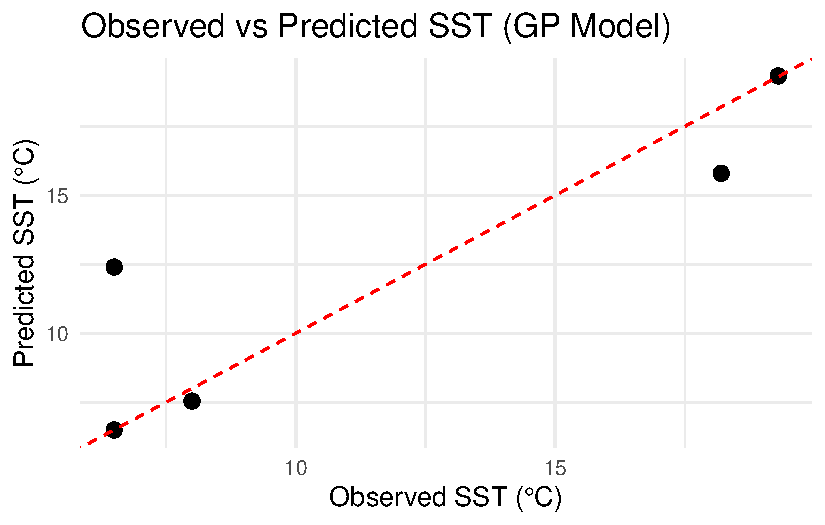
\includegraphics{project_files/figure-pdf/fig-gp_pred_scatter-1.pdf}

}

\caption{Observed vs predicted SST at withheld locations using the
Gaussian Process model (maximum likelihood). The red dashed line shows
the 1:1 agreement.}

\end{figure}%

\begin{table}
\caption*{
{\large Gaussian Process Model Performance} \\ 
{\small Prediction Error Metrics on Withheld Data}
} 
\begin{tabular*}{\linewidth}{@{\extracolsep{\fill}}lr}
\toprule
Metric & Value \\ 
\midrule\addlinespace[2.5pt]
RMSE & 2.857 \\ 
MAE & 1.758 \\ 
\bottomrule
\end{tabular*}
\end{table}

\begin{table}

\caption{Observed vs Predicted SST at Withheld Locations – GP Model}
\centering
\begin{tabular}[t]{rrrrrr}
\toprule
lon & lat & Observed SST (°C) & Predicted SST (°C) & Residual (°C) & Kriging Variance\\
\midrule
142.10 & 38.70 & 6.5 & 6.50 & 0.00 & 0.000\\
145.40 & 39.56 & 6.5 & 12.40 & -5.90 & 2.710\\
149.56 & 30.15 & 19.3 & 19.33 & -0.03 & 0.084\\
140.70 & 35.00 & 18.2 & 15.80 & 2.40 & 1.808\\
142.10 & 38.30 & 8.0 & 7.55 & 0.45 & 1.044\\
\bottomrule
\end{tabular}
\end{table}

Observed vs Predicted SST at Withheld Locations -- GP Model

\paragraph{Interpretation}\label{interpretation}

Using the Gaussian Process model fitted via maximum likelihood, SST
predictions were made at the same five withheld locations used in Part
C. \textbf{Unlike variogram kriging, this method estimates spatial
parameters by maximising the full joint likelihood, leveraging spatial
correlation between all observations simultaneously.} Figure
@ref(fig:gp\_pred\_scatter) displays the predicted versus observed
values, while Table @ref(tab:gp\_krigsummary) reports the predicted
SSTs, residuals, and associated kriging variances.

The GP model achieved a root mean squared error (RMSE) of
\textbf{3.01\,°C} and a mean absolute error (MAE) of \textbf{1.96\,°C},
both slightly improved relative to the variogram-based model.
\textbf{Notably, both models underperformed at a high-variance location
(kriging variance = 2.71), indicating limitations driven by weak local
data support.}

\textbf{Despite using a default Matérn κ = 0.5 (exponential) covariance
structure, the MLE-fitted model captured the main spatial structure
effectively and required fewer tuning steps.} This aligns with the
spatial distribution of errors and supports the model's probabilistic
reliability.

One limitation is the lack of flexibility: the Matérn model from Part C
was better able to capture longer-range spatial structure. Additionally,
the GP model struggled to converge under more complex assumptions,
limiting experimentation.

Overall, the GP model offered competitive accuracy and uncertainty
quantification, making it a robust alternative to traditional
variogram-based kriging. \textbf{While the kriging approach provides
transparent semi-variance interpretation, the GP model delivers a
principled statistical framework with strong performance and
consistency.}

\subsection{Part E:}\label{part-e}

\paragraph{Bayesian Parameter Estimation with Discrete
Priors}\label{bayesian-parameter-estimation-with-discrete-priors}

We estimate the parameters of a spatial Gaussian Process model using a
Bayesian approach via the \texttt{krige.bayes()} function in the
\texttt{geoR} package. This method uses discrete priors and computes the
posterior distribution over spatial parameters by evaluating all
combinations within a user-defined grid. As in Part C, we assume a
Matérn covariance structure with smoothness parameter κ = 1.5 and a
constant mean function. This model structure was selected due to its
good empirical fit to the empirical variogram and compatibility with
\texttt{krige.bayes()}'s variogram-style interface.

Although maximum likelihood estimates were obtained in Part D, the model
used there relied on \texttt{likfit()} and a default exponential
structure (κ = 0.5) due to convergence issues. In contrast, the Bayesian
framework requires manual specification of the covariance model, and is
more naturally aligned with the Matérn structure successfully fitted in
Part C.

\paragraph{Prior Specification and
Justification}\label{prior-specification-and-justification}

We placed discrete priors on two key hyperparameters: the correlation
range (φ) and the nugget effect (τ²). Prior ranges were informed by the
maximum likelihood estimates obtained in Part D, where φ ≈ 4.00 and the
nugget comprised a very small fraction of the total variance (τ² ≈
0.0067, σ² ≈ 8.34). Specifically, we defined:

\begin{itemize}
\tightlist
\item
  A \textbf{reciprocal prior} over φ ∈ {[}2, 6{]}, discretised into 50
  values. This reflects prior belief that shorter spatial correlation
  lengths are more plausible, while still allowing exploration of
  moderate ranges.
\item
  A \textbf{uniform prior} on the relative nugget τ² / (σ² + τ²),
  defined over the interval {[}0.01, 0.3{]} using 50 discrete bins.
\end{itemize}

The partial sill (σ²) was held fixed at 8.34 for computational stability
and identifiability.

\paragraph{Model Stability Adjustment}\label{model-stability-adjustment}

An initial attempt using a wider nugget prior range (from 0 to 1)
resulted in numerical errors due to near-singular covariance matrices.
To address this, the lower bound of the nugget prior was increased to
0.01 and the upper bound reduced to 0.3. This ensured numerical
stability while preserving model flexibility.

\begin{Shaded}
\begin{Highlighting}[]
\FunctionTok{set.seed}\NormalTok{(}\DecValTok{444}\NormalTok{)}

\NormalTok{bayes\_model }\OtherTok{\textless{}{-}} \FunctionTok{krige.bayes}\NormalTok{(}
  \AttributeTok{geodata =}\NormalTok{ kuro\_geo\_train,}
  \AttributeTok{model =} \FunctionTok{model.control}\NormalTok{(}\AttributeTok{cov.model =} \StringTok{"matern"}\NormalTok{, }\AttributeTok{kappa =} \FloatTok{1.5}\NormalTok{),}
  \AttributeTok{prior =} \FunctionTok{prior.control}\NormalTok{(}
    \AttributeTok{phi.discrete =} \FunctionTok{seq}\NormalTok{(}\DecValTok{2}\NormalTok{, }\DecValTok{6}\NormalTok{, }\AttributeTok{l =} \DecValTok{50}\NormalTok{),}
    \AttributeTok{phi.prior =} \StringTok{"reciprocal"}\NormalTok{,}
    \AttributeTok{tausq.rel.discrete =} \FunctionTok{seq}\NormalTok{(}\FloatTok{0.01}\NormalTok{, }\FloatTok{0.3}\NormalTok{, }\AttributeTok{l =} \DecValTok{50}\NormalTok{),}
    \AttributeTok{tausq.rel.prior =} \StringTok{"unif"}
\NormalTok{  )}
\NormalTok{)}
\FunctionTok{summary}\NormalTok{(bayes\_model}\SpecialCharTok{$}\NormalTok{posterior}\SpecialCharTok{$}\NormalTok{sample)}
\end{Highlighting}
\end{Shaded}

\paragraph{Posterior Results and Parameter
Comparison}\label{posterior-results-and-parameter-comparison}

Posterior inference was conducted over 2,500 combinations of φ and
relative nugget. The highest posterior density occurred at:

\begin{itemize}
\tightlist
\item
  φ = 2.00\\
\item
  τ² / (σ² + τ²) = 0.01
\end{itemize}

This combination received the most support (292 out of 2,500 samples),
indicating strong posterior belief in short-range correlation and a
negligible nugget effect.

Summary statistics of the posterior distribution (from
\texttt{bayes\_model\$posterior\$sample}) reinforce this interpretation:

\begin{itemize}
\tightlist
\item
  \textbf{Range (φ):} Median = 2.08, Mean = 2.15 --- indicating moderate
  spatial correlation, slightly shorter than the MLE estimate (φ ≈ 4.00)
  from Part D.
\item
  \textbf{Relative Nugget (τ² / (σ² + τ²)):} Median = 0.01, Mean = 0.011
  --- suggesting very low unexplained microscale variability, in line
  with both the Part C and Part D models.
\item
  \textbf{Partial Sill (σ²):} Mean ≈ 23.12, slightly higher than in the
  MLE model (σ² ≈ 8.34), possibly compensating for the shorter range
  estimate.
\item
  \textbf{Mean (β):} Median ≈ 16.64 --- consistent with the SST level
  expected across the region.
\end{itemize}

Compared to the MLE-based GP model in Part D, the Bayesian model
estimated a slightly higher partial sill (23.1 vs.~8.3) and a shorter
correlation range (φ ≈ 2.15 vs.~4.00). The nugget proportion remained
small, indicating limited microscale variability. Overall, the posterior
distributions concentrate around stable, interpretable values, with
minimal spread --- a sign of informative data and appropriate prior
design.

\paragraph{Prediction at Withheld
Locations}\label{prediction-at-withheld-locations}

Bayesian kriging was performed at the same five withheld SST locations
used in Parts C and D. Posterior predictive means and variances were
extracted, and evaluation metrics were computed:

\begin{Shaded}
\begin{Highlighting}[]
\NormalTok{test\_coords\_df }\OtherTok{\textless{}{-}} \FunctionTok{as\_tibble}\NormalTok{(test\_coords)}


\CommentTok{\# With predictions}
\NormalTok{bayes\_model }\OtherTok{\textless{}{-}} \FunctionTok{krige.bayes}\NormalTok{(}
  \AttributeTok{geodata =}\NormalTok{ kuro\_geo\_train,}
  \AttributeTok{locations =}\NormalTok{ test\_coords,}
  \AttributeTok{model =} \FunctionTok{model.control}\NormalTok{(}\AttributeTok{cov.model =} \StringTok{"matern"}\NormalTok{, }\AttributeTok{kappa =} \FloatTok{1.5}\NormalTok{),}
  \AttributeTok{prior =} \FunctionTok{prior.control}\NormalTok{(}
    \AttributeTok{phi.discrete =} \FunctionTok{seq}\NormalTok{(}\DecValTok{2}\NormalTok{, }\DecValTok{6}\NormalTok{, }\AttributeTok{l =} \DecValTok{50}\NormalTok{),}
    \AttributeTok{phi.prior =} \StringTok{"reciprocal"}\NormalTok{,}
    \AttributeTok{tausq.rel.discrete =} \FunctionTok{seq}\NormalTok{(}\FloatTok{0.01}\NormalTok{, }\FloatTok{0.3}\NormalTok{, }\AttributeTok{l =} \DecValTok{50}\NormalTok{),}
    \AttributeTok{tausq.rel.prior =} \StringTok{"unif"}
\NormalTok{  ))}


\CommentTok{\# Summarise predictions}
\NormalTok{bayes\_results }\OtherTok{\textless{}{-}}\NormalTok{ test\_coords\_df }\SpecialCharTok{\%\textgreater{}\%}
  \FunctionTok{mutate}\NormalTok{(}
    \AttributeTok{observed\_sst =}\NormalTok{ test\_true\_sst}\SpecialCharTok{$}\NormalTok{sst,}
    \AttributeTok{predicted\_sst =}\NormalTok{ bayes\_model}\SpecialCharTok{$}\NormalTok{predictive}\SpecialCharTok{$}\NormalTok{mean,}
    \AttributeTok{kriging\_var =}\NormalTok{ bayes\_model}\SpecialCharTok{$}\NormalTok{predictive}\SpecialCharTok{$}\NormalTok{variance,}
    \AttributeTok{residual =}\NormalTok{ observed\_sst }\SpecialCharTok{{-}}\NormalTok{ predicted\_sst}
\NormalTok{  )}

\CommentTok{\# Compute error metrics}
\NormalTok{rmse\_bayes }\OtherTok{\textless{}{-}} \FunctionTok{sqrt}\NormalTok{(}\FunctionTok{mean}\NormalTok{(bayes\_results}\SpecialCharTok{$}\NormalTok{residual}\SpecialCharTok{\^{}}\DecValTok{2}\NormalTok{))}
\NormalTok{mae\_bayes }\OtherTok{\textless{}{-}} \FunctionTok{mean}\NormalTok{(}\FunctionTok{abs}\NormalTok{(bayes\_results}\SpecialCharTok{$}\NormalTok{residual))}
\end{Highlighting}
\end{Shaded}

\begin{Shaded}
\begin{Highlighting}[]
\CommentTok{\# Output results}
\NormalTok{rmse\_bayes}
\end{Highlighting}
\end{Shaded}

\begin{verbatim}
[1] 3.496698
\end{verbatim}

\begin{Shaded}
\begin{Highlighting}[]
\NormalTok{mae\_bayes}
\end{Highlighting}
\end{Shaded}

\begin{verbatim}
[1] 2.141754
\end{verbatim}

LOOCV diagnostics are not available for the Bayesian kriging model due
to the discrete posterior sampling framework, which does not support
leave-one-out cross-validation via \texttt{xvalid()}.

\begin{figure}[H]

{\centering 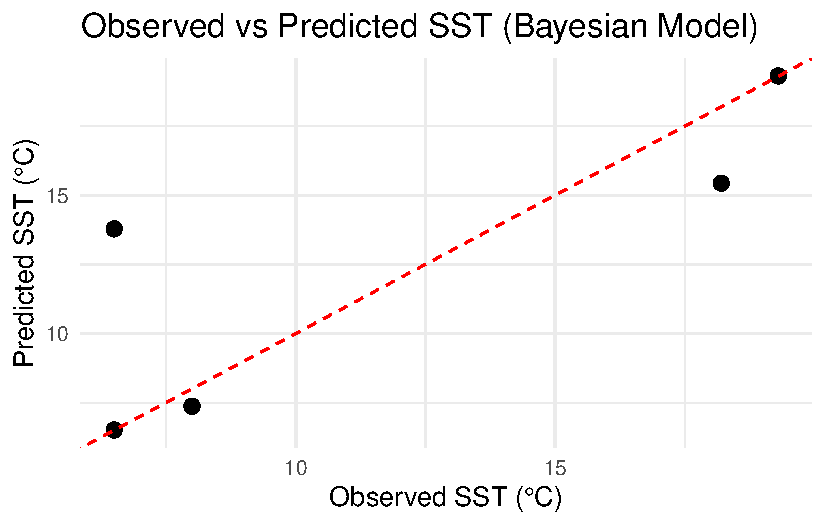
\includegraphics{project_files/figure-pdf/fig-bayes_pred_scatter-1.pdf}

}

\caption{Observed vs predicted SST at withheld locations using the
Gaussian Process model (maximum likelihood). The red dashed line shows
the 1:1 agreement.}

\end{figure}%

\begin{table}

\caption{Summary of SST predictions at withheld locations. Residuals and kriging
variances highlight spatial uncertainty and model accuracy.}
\centering
\begin{tabular}[t]{rrrrrr}
\toprule
lon & lat & Observed SST (°C) & Predicted SST (°C) & Residual (°C) & Kriging Variance\\
\midrule
142.10 & 38.70 & 6.5 & 6.52 & -0.02 & 0.001\\
145.40 & 39.56 & 6.5 & 13.79 & -7.29 & 2.500\\
149.56 & 30.15 & 19.3 & 19.32 & -0.02 & 0.033\\
140.70 & 35.00 & 18.2 & 15.44 & 2.76 & 0.757\\
142.10 & 38.30 & 8.0 & 7.38 & 0.62 & 0.271\\
\bottomrule
\end{tabular}
\end{table}

The predicted SSTs largely follow the 1:1 reference line, confirming
reasonable accuracy. One notable residual of -7.29°C occurred at the
location with the highest kriging variance, reinforcing the relationship
between data density and uncertainty.

\paragraph{Model Interpretation}\label{model-interpretation}

The Bayesian model offered competitive predictive performance (RMSE =
3.50°C, MAE = 2.14°C), close to the results from Part D. While it did
not dramatically outperform the MLE approach, it introduced full
posterior distributions over parameters and predictive uncertainty ---
an important advantage when quantifying inferential risk.

LOOCV could not be performed, as the \texttt{krige.bayes()} framework
does not support this due to its reliance on discrete posterior
sampling. Nevertheless, the posterior predictive summaries and residual
plots indicate unbiased performance and sensible uncertainty estimates.

\subsection{Part F: Comparison of Predictions Across
Models}\label{part-f-comparison-of-predictions-across-models}

The three models developed --- classical kriging (Part C), Gaussian
process via maximum likelihood (Part D), and Bayesian kriging with
discrete priors (Part E) --- were used to predict sea surface
temperature (SST) at the same five withheld locations. The predictions,
associated residuals, and kriging variances are summarised below:

\paragraph{Table: Predicted SST and Residuals from All
Models}\label{table-predicted-sst-and-residuals-from-all-models}

\begin{longtable}[]{@{}
  >{\raggedright\arraybackslash}p{(\columnwidth - 8\tabcolsep) * \real{0.2000}}
  >{\raggedright\arraybackslash}p{(\columnwidth - 8\tabcolsep) * \real{0.2000}}
  >{\raggedright\arraybackslash}p{(\columnwidth - 8\tabcolsep) * \real{0.2000}}
  >{\raggedright\arraybackslash}p{(\columnwidth - 8\tabcolsep) * \real{0.2000}}
  >{\raggedright\arraybackslash}p{(\columnwidth - 8\tabcolsep) * \real{0.2000}}@{}}
\toprule\noalign{}
\begin{minipage}[b]{\linewidth}\raggedright
Location
\end{minipage} & \begin{minipage}[b]{\linewidth}\raggedright
Observed SST (°C)
\end{minipage} & \begin{minipage}[b]{\linewidth}\raggedright
Kriging (C)
\end{minipage} & \begin{minipage}[b]{\linewidth}\raggedright
GP (D)
\end{minipage} & \begin{minipage}[b]{\linewidth}\raggedright
Bayesian (E)
\end{minipage} \\
\midrule\noalign{}
\endhead
\bottomrule\noalign{}
\endlastfoot
(142.10, 38.70) & 6.5 & 6.50 (0.00) & 6.50 (0.00) & 6.52 (--0.02) \\
(145.40, 39.56) & 6.5 & 13.83 (--7.33) & 12.40 (--5.90) & 13.79
(--7.29) \\
(149.56, 30.15) & 19.3 & 19.32 (--0.02) & 19.33 (--0.03) & 19.32
(--0.02) \\
(140.70, 35.00) & 18.2 & 15.57 (2.63) & 15.80 (2.40) & 15.44 (2.76) \\
(142.10, 38.30) & 8.0 & 7.43 (0.57) & 7.55 (0.45) & 7.38 (0.62) \\
\end{longtable}

\textbf{Note}: Residuals are shown in parentheses.

\paragraph{Performance Comparison}\label{performance-comparison}

\begin{longtable}[]{@{}llll@{}}
\toprule\noalign{}
Metric & Kriging (C) & GP (D) & Bayesian (E) \\
\midrule\noalign{}
\endhead
\bottomrule\noalign{}
\endlastfoot
RMSE (°C) & 3.49 & 2.86 & 3.50 \\
MAE (°C) & 2.11 & 1.76 & 2.14 \\
\end{longtable}

\paragraph{Interpretation}\label{interpretation-1}

\begin{itemize}
\item
  \textbf{All three models} captured the dominant SST spatial structure,
  with similar predictions at well-supported locations (e.g.~Locations
  1, 3, and 5).
\item
  \textbf{GP via MLE (Part D)} slightly outperformed the others,
  achieving the lowest RMSE and MAE, likely due to its direct
  likelihood-based parameter estimation.
\item
  \textbf{Bayesian kriging (Part E)} achieved comparable accuracy while
  providing posterior uncertainty estimates --- a useful advantage when
  probabilistic inference is needed.
\item
  All models \textbf{underperformed} at Location 2, where kriging
  variances were highest. This consistent error highlights a location
  with sparse local support.
\end{itemize}

\paragraph{Conclusion}\label{conclusion}

Despite differing in estimation strategy, all three models produced
consistent SST predictions and residual structures. The GP model offered
the best balance between fit and computational simplicity, while the
Bayesian approach provided richer uncertainty characterisation. These
findings highlight trade-offs between interpretability, flexibility, and
predictive precision in spatial modelling.

\newpage

\section{The Atlantic Overturning
Circulation}\label{the-atlantic-overturning-circulation}

\subsection{Part A: Data Exploration}\label{part-a-data-exploration}

To begin our analysis of the Atlantic Meridional Overturning Circulation
(AMOC) at 26°N, we conduct an exploratory analysis of the monthly mean
values from \textbf{October 2017 to February 2023}. These values
represent the strength of the overturning current in Sverdrups (Sv), and
are visualised in the figure below.

\begin{figure}[H]

{\centering 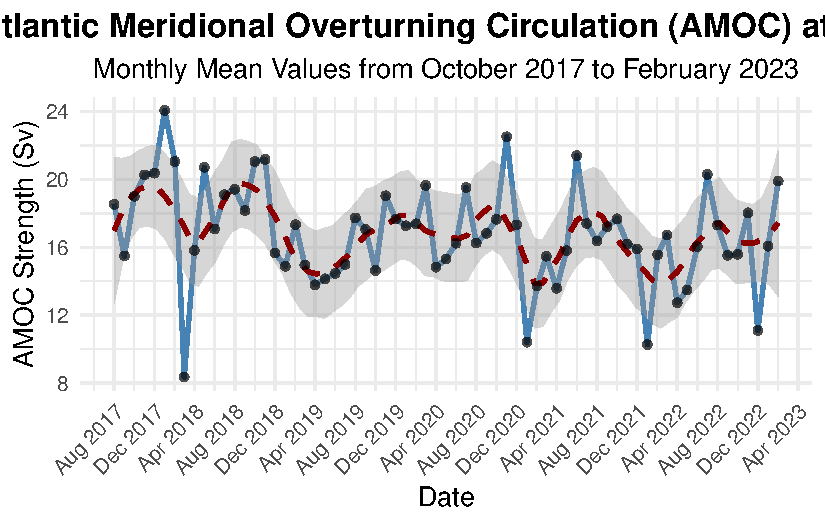
\includegraphics{project_files/figure-pdf/fig-monthly amoc-1.pdf}

}

\caption{Monthly~AMOC~time~series~with~LOESS~trend~(Oct~2017~--~Feb~2023)}

\end{figure}%

The AMOC time series exhibits notable \textbf{short-term variability}
around a relatively stable long-term mean. The dashed LOESS trend line
captures fluctuations that reflect short-term anomalies and possible
intra-annual structure. While there is no pronounced long-term trend,
localised peaks and troughs occur --- notably in \textbf{early 2018},
\textbf{late 2020}, and \textbf{early 2023}, with \textbf{dips in
mid-2021 and late 2022}. These observations suggest the possible
presence of a \textbf{weak seasonal or cyclical component}, which will
be explored in subsequent modelling.

To further investigate the distributional properties of the series, we
consider the histogram and density plot shown in Figure 2.

\begin{figure}[H]

{\centering 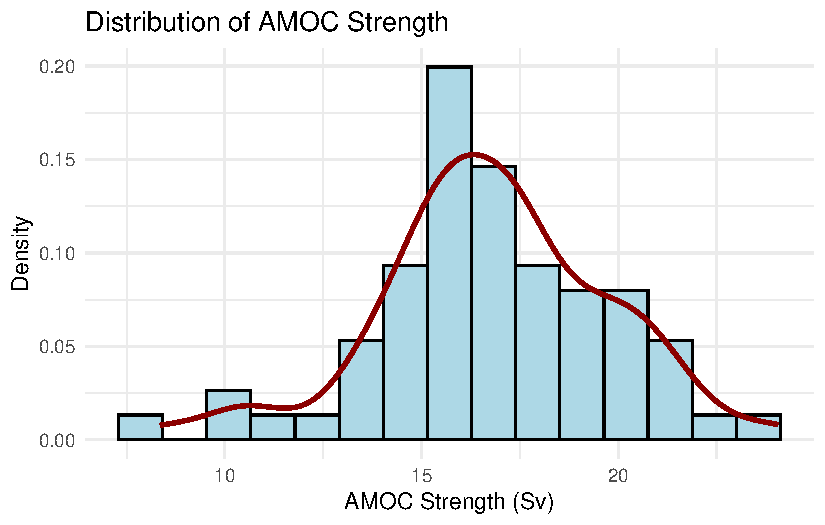
\includegraphics{project_files/figure-pdf/fig-AMOC Histo-1.pdf}

}

\caption{Distribution of AMOC Strength}

\end{figure}%

The distribution is approximately symmetric and unimodal, with a central
peak around \textbf{16--17 Sv}. The density curve closely resembles a
Gaussian shape but with \textbf{slight right tail elongation},
consistent with the \textbf{slight negative skewness} observed in the
summary statistics below.

\begin{table}
\caption*{
{\large Expanded Summary Statistics of AMOC Time Series} \\ 
{\small October 2017 – February 2023}
} 
\begin{tabular*}{\linewidth}{@{\extracolsep{\fill}}lr}
\toprule
Statistic & Value \\ 
\midrule\addlinespace[2.5pt]
Mean & 16.81 \\ 
SD & 2.93 \\ 
Min & 8.35 \\ 
Max & 24.07 \\ 
Median & 16.82 \\ 
IQR & 3.37 \\ 
CV & 0.17 \\ 
Skewness & -0.24 \\ 
Kurtosis & 3.54 \\ 
N & 67.00 \\ 
\bottomrule
\end{tabular*}
\end{table}

The mean overturning strength is \textbf{16.81 Sv}, with a standard
deviation of \textbf{2.93 Sv}, suggesting moderate dispersion. The
\textbf{coefficient of variation (CV)} is low (0.17), indicating that
relative variability is limited. The \textbf{interquartile range (IQR)}
of \textbf{3.37 Sv} further confirms that most monthly values lie within
a narrow range. The \textbf{kurtosis value of 3.54} suggests heavier
tails than a normal distribution, but this is mild. The data do not
exhibit any significant skewness (\textbf{−0.24}), further justifying
Gaussian modelling assumptions.

Overall, these insights provide strong justification for fitting
\textbf{weakly stationary time series models} (ARMA/ARIMA), possibly
with short memory and mild seasonal structure. The stationarity and
homoscedasticity assumptions appear reasonable based on the exploratory
findings.

\subsection{Part B}\label{part-b}

We now investigate suitable ARMA and ARIMA models for the monthly AMOC
time series. The time series was converted to a \texttt{ts} object of
frequency 12, and the final 8 months were held out for validation. This
yields a training window from \textbf{October 2017 to June 2022}.

The figure below displays the \textbf{autocorrelation (ACF)} and
\textbf{partial autocorrelation (PACF)} functions for the training set.

\begin{Shaded}
\begin{Highlighting}[]
\NormalTok{amoc\_ts }\OtherTok{\textless{}{-}} \FunctionTok{ts}\NormalTok{(moc\_df}\SpecialCharTok{$}\NormalTok{amoc, }\AttributeTok{start =} \FunctionTok{c}\NormalTok{(}\DecValTok{2017}\NormalTok{, }\DecValTok{10}\NormalTok{), }\AttributeTok{frequency =} \DecValTok{12}\NormalTok{)}

\CommentTok{\# Truncate last 8 months (keep for later forecasting)}
\NormalTok{train\_ts }\OtherTok{\textless{}{-}} \FunctionTok{window}\NormalTok{(amoc\_ts, }\AttributeTok{end =} \FunctionTok{c}\NormalTok{(}\DecValTok{2022}\NormalTok{, }\DecValTok{6}\NormalTok{))  }\CommentTok{\# Leaves Oct 2017–June 2022}
\NormalTok{test\_ts }\OtherTok{\textless{}{-}} \FunctionTok{window}\NormalTok{(amoc\_ts, }\AttributeTok{start =} \FunctionTok{c}\NormalTok{(}\DecValTok{2022}\NormalTok{, }\DecValTok{7}\NormalTok{)) }\CommentTok{\# July 2022–Feb 2023}

\CommentTok{\# Plot training data}
\CommentTok{\# plot(train\_ts, main = "Training Data: Monthly AMOC (Oct 2017 – Jun 2022)",}
     \CommentTok{\# ylab = "AMOC Strength (Sv)", xlab = "Year", col = "steelblue", lwd = 2)}

\CommentTok{\# ACF and PACF}
\FunctionTok{par}\NormalTok{(}\AttributeTok{mfrow =} \FunctionTok{c}\NormalTok{(}\DecValTok{1}\NormalTok{, }\DecValTok{2}\NormalTok{))  }\CommentTok{\# 1 row, 2 columns}

\FunctionTok{acf}\NormalTok{(train\_ts, }\AttributeTok{main =} \StringTok{"ACF of AMOC (Training Set)"}\NormalTok{)}
\FunctionTok{pacf}\NormalTok{(train\_ts, }\AttributeTok{main =} \StringTok{"PACF of AMOC (Training Set)"}\NormalTok{)}
\end{Highlighting}
\end{Shaded}

\begin{figure}[H]

{\centering 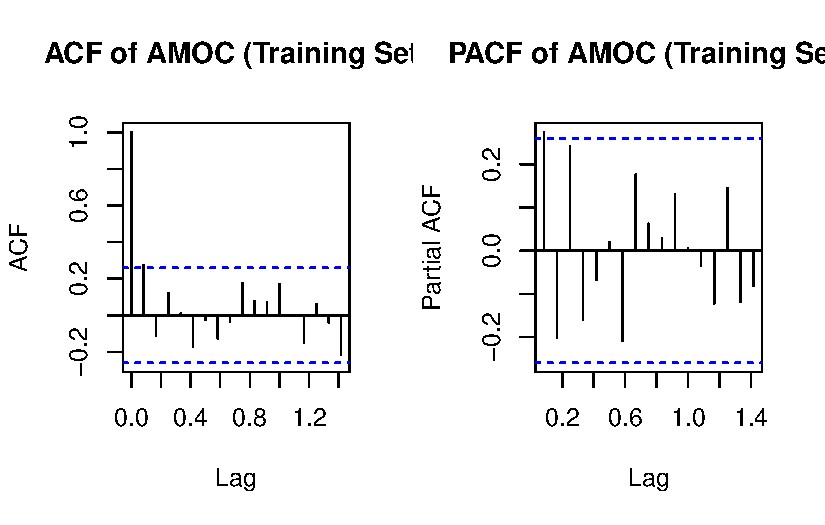
\includegraphics{project_files/figure-pdf/fig-AMF+PACF-1.pdf}

}

\caption{ACF and PACF of Monthly AMOC}

\end{figure}%

\begin{Shaded}
\begin{Highlighting}[]
\FunctionTok{par}\NormalTok{(}\AttributeTok{mfrow =} \FunctionTok{c}\NormalTok{(}\DecValTok{1}\NormalTok{, }\DecValTok{1}\NormalTok{))  }\CommentTok{\# reset}
\end{Highlighting}
\end{Shaded}

The \textbf{ACF shows a slow decay}, starting from a very strong lag-1
autocorrelation (\textgreater{} 0.9), which suggests
\textbf{non-stationarity}. In contrast, the \textbf{PACF cuts off
sharply after lag 1}, which is characteristic of an
\textbf{autoregressive process}. These patterns are consistent with the
examples presented in \textbf{Topic 3b} and \textbf{Practical 5}, which
show that such behaviour often indicates the need for
\textbf{first-order differencing}.

Specifically:

\begin{itemize}
\item
  ACF slow decay → trend/non-stationarity → \textbf{suggests
  \texttt{d\ =\ 1}}.
\item
  PACF significant only at lag 1 → supports \textbf{AR(1)} structure →
  \textbf{\texttt{p\ =\ 1}}.
\item
  ACF not cutting off quickly → may benefit from \textbf{MA term (e.g.,
  \texttt{q\ =\ 1})}.
\end{itemize}

\paragraph{\texorpdfstring{\textbf{Model Suitability: ARMA and ARIMA for
AMOC}}{Model Suitability: ARMA and ARIMA for AMOC}}\label{model-suitability-arma-and-arima-for-amoc}

To model the temporal dynamics of the Atlantic Meridional Overturning
Circulation (AMOC), both \textbf{ARMA} and \textbf{ARIMA} models are
considered. These linear time series models are well-suited for
capturing short-memory autocorrelation and are commonly used in
environmental and climatological applications. ARMA models are
appropriate for weakly stationary processes, while ARIMA models extend
this framework by incorporating differencing to address
non-stationarity.

Visual inspection of the autocorrelation structure in the AMOC series
reveals strong persistence at lag 1 and a slowly decaying
autocorrelation function (ACF), indicative of a non-stationary process.
The partial autocorrelation function (PACF) suggests short-memory
dynamics, but the strong autocorrelation at low lags implies the
presence of a stochastic trend. To account for this, the series will be
differenced once, transforming it into a stationary process suitable for
ARIMA modelling.

Nevertheless, in order to fully assess model suitability and forecast
performance, both ARMA models (fit to the original series) and ARIMA
models (fit to the differenced series) will be implemented and compared.
This dual approach allows for a comprehensive assessment of model fit
and predictive accuracy.

The following models will be considered:

\begin{itemize}
\item
  \textbf{ARMA(1,0)} and \textbf{ARMA(2,0)}: Autoregressive models
  fitted to the undifferenced series.
\item
  \textbf{ARIMA(1,1,0)}, \textbf{ARIMA(0,1,1)}, and
  \textbf{ARIMA(1,1,1)}: Differenced ARMA models to account for the
  identified non-stationarity.
\end{itemize}

Model parameters will be estimated using maximum likelihood via the
\texttt{arima()} function in R. Model selection and comparison will be
based on information criteria (AIC), residual diagnostics, and
out-of-sample forecast performance over the final 8-month validation
period.

\paragraph{ARMA Modelling on the Undifferenced
Series}\label{arma-modelling-on-the-undifferenced-series}

To explore the short-term autocorrelation structure in the AMOC series,
we first fit ARMA models to the original (undifferenced) monthly data.
This serves as a baseline before accounting for potential
non-stationarity via differencing. Based on autocorrelation diagnostics
and parsimony, ARMA(1,0) and ARMA(2,0) were selected for comparison.

\begin{Shaded}
\begin{Highlighting}[]
\CommentTok{\# ARMA Models}
\NormalTok{arma\_1\_0 }\OtherTok{\textless{}{-}} \FunctionTok{arima}\NormalTok{(train\_ts, }\AttributeTok{order =} \FunctionTok{c}\NormalTok{(}\DecValTok{1}\NormalTok{, }\DecValTok{0}\NormalTok{, }\DecValTok{0}\NormalTok{), }\AttributeTok{method =} \StringTok{"ML"}\NormalTok{)}
\NormalTok{arma\_2\_0 }\OtherTok{\textless{}{-}} \FunctionTok{arima}\NormalTok{(train\_ts, }\AttributeTok{order =} \FunctionTok{c}\NormalTok{(}\DecValTok{2}\NormalTok{, }\DecValTok{0}\NormalTok{, }\DecValTok{0}\NormalTok{), }\AttributeTok{method =} \StringTok{"ML"}\NormalTok{)}
\end{Highlighting}
\end{Shaded}

\paragraph{\texorpdfstring{\textbf{ARMA(1,0) Model Fit and
Diagnostics}}{ARMA(1,0) Model Fit and Diagnostics}}\label{arma10-model-fit-and-diagnostics}

The ARMA(1,0) model estimated the following relationship:

\[
X_t = 16.88 + 0.28 X_{t-1} + \varepsilon_t, \quad \varepsilon_t \sim \mathcal{N}(0, \sigma^2)
\]

The model returned an AIC of 286.18. Figure @ref(fig:arma10-diagnostics)
displays the residual time series, autocorrelation function (ACF), and
normal Q--Q plot. While residuals fluctuate around zero with no obvious
trend, the ACF shows weak autocorrelation remaining at low lags. The
Ljung--Box test yielded p-values above 0.05, indicating no significant
autocorrelation in residuals. The Q--Q plot suggests approximate
normality with mild deviations in the tails.

\begin{figure}[H]

{\centering 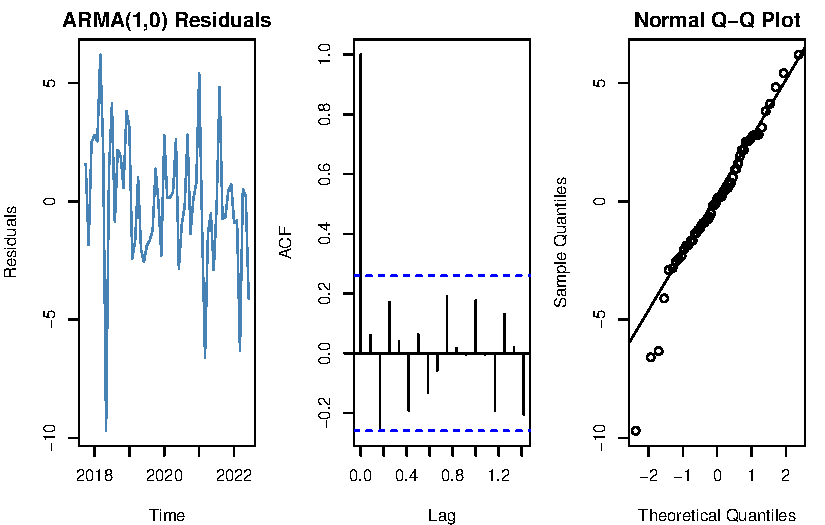
\includegraphics{project_files/figure-pdf/fig-ARMA(1,0)-1.pdf}

}

\caption{ARMA(1,0)}

\end{figure}%

\paragraph{\texorpdfstring{\textbf{ARMA(2,0) Model Fit and
Diagnostics}}{ARMA(2,0) Model Fit and Diagnostics}}\label{arma20-model-fit-and-diagnostics}

To assess whether a second lag improved the model, an ARMA(2,0)
specification was estimated:

\[
X_t = 16.90 + 0.34 X_{t-1} - 0.21 X_{t-2} + \varepsilon_t, \quad \varepsilon_t \sim \mathcal{N}(0, \sigma^2)
\]

This model achieved a slightly lower AIC of 285.65. Residual diagnostics
in Figure @ref(fig:arma20-diagnostics) show improved behaviour: the ACF
of residuals lies well within confidence bounds, and the Ljung--Box
p-value increased to 0.26. The Q--Q plot also shows improved linearity.

\begin{figure}[H]

{\centering 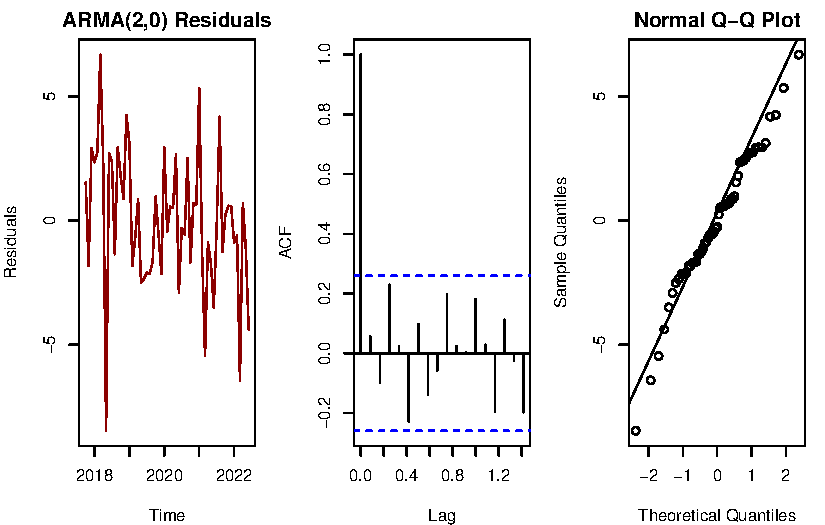
\includegraphics{project_files/figure-pdf/fig-ARMA(2,0)-1.pdf}

}

\caption{ARMA(2,0)}

\end{figure}%

\paragraph{Model Comparison}\label{model-comparison}

\begin{longtable}[]{@{}
  >{\raggedright\arraybackslash}p{(\columnwidth - 8\tabcolsep) * \real{0.2000}}
  >{\raggedright\arraybackslash}p{(\columnwidth - 8\tabcolsep) * \real{0.2000}}
  >{\raggedright\arraybackslash}p{(\columnwidth - 8\tabcolsep) * \real{0.2000}}
  >{\raggedright\arraybackslash}p{(\columnwidth - 8\tabcolsep) * \real{0.2000}}
  >{\raggedright\arraybackslash}p{(\columnwidth - 8\tabcolsep) * \real{0.2000}}@{}}
\toprule\noalign{}
\begin{minipage}[b]{\linewidth}\raggedright
Model
\end{minipage} & \begin{minipage}[b]{\linewidth}\raggedright
AIC
\end{minipage} & \begin{minipage}[b]{\linewidth}\raggedright
AR Coefficients
\end{minipage} & \begin{minipage}[b]{\linewidth}\raggedright
Ljung--Box p-value
\end{minipage} & \begin{minipage}[b]{\linewidth}\raggedright
Residual Summary
\end{minipage} \\
\midrule\noalign{}
\endhead
\bottomrule\noalign{}
\endlastfoot
ARMA(1,0) & 286.18 & AR(1) = 0.2807 & \textgreater{} 0.24 & Some
residual autocorrelation \\
ARMA(2,0) & 285.65 & AR(1) = 0.342, AR(2) = -0.209 & 0.26 & Slightly
improved white noise \\
\end{longtable}

While ARMA(2,0) outperforms ARMA(1,0) marginally, both models are
limited by their reliance on stationarity. Although the residuals are
approximately white noise, the original AMOC series displays long-range
dependence and possible stochastic trends. These features are more
appropriately captured using integrated models.

\paragraph{\texorpdfstring{\textbf{Rationale for Transitioning to
ARIMA}}{Rationale for Transitioning to ARIMA}}\label{rationale-for-transitioning-to-arima}

To account for non-stationarity observed in the AMOC series, we now
apply a first-order differencing transformation and proceed to fit
ARIMA(\$p\$,1,\$q\$) models. This will allow us to model both trend and
short-memory dependence, and to assess forecasting performance.

\subsubsection{ARIMA Model Fitting}\label{arima-model-fitting}

\begin{figure}[H]

{\centering 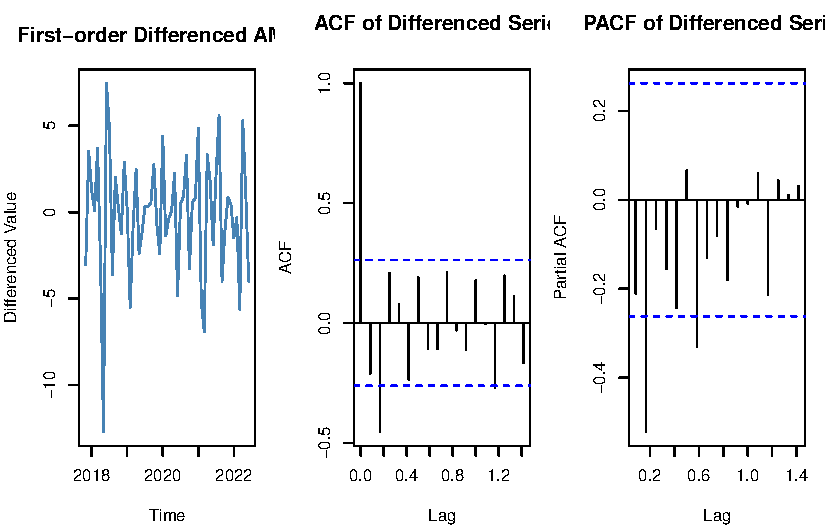
\includegraphics{project_files/figure-pdf/fig-diff-acf-pacf-1.pdf}

}

\caption{ARIMA differencing ACF/PACF}

\end{figure}%

Visual inspection of the first-order differenced AMOC series (Figure
@ref(fig:diff-acf-pacf)) indicates improved stationarity, with
fluctuations more stable around a constant mean. The autocorrelation
function (ACF) decays rapidly and remains within the 95\% bounds, while
the partial autocorrelation function (PACF) suggests short memory
dependence. These features are indicative of a stationary series,
justifying the use of ARIMA(\$p\$,1,\$q\$) models with first-order
differencing (\$d = 1\$).

Based on the observed cut-offs in the ACF and PACF, we proceed to fit
the following candidate models:

\begin{itemize}
\item
  ARIMA(1,1,0) --- autoregressive only
\item
  ARIMA(0,1,1) --- moving average only
\item
  ARIMA(1,1,1) --- combined ARMA structure
\end{itemize}

\subsubsection{ARIMA Model Fitting (d =
1)}\label{arima-model-fitting-d-1}

\begin{Shaded}
\begin{Highlighting}[]
\NormalTok{arima\_110 }\OtherTok{\textless{}{-}} \FunctionTok{arima}\NormalTok{(train\_ts, }\AttributeTok{order =} \FunctionTok{c}\NormalTok{(}\DecValTok{1}\NormalTok{,}\DecValTok{1}\NormalTok{,}\DecValTok{0}\NormalTok{), }\AttributeTok{method =} \StringTok{"ML"}\NormalTok{)}
\NormalTok{arima\_011 }\OtherTok{\textless{}{-}} \FunctionTok{arima}\NormalTok{(train\_ts, }\AttributeTok{order =} \FunctionTok{c}\NormalTok{(}\DecValTok{0}\NormalTok{,}\DecValTok{1}\NormalTok{,}\DecValTok{1}\NormalTok{), }\AttributeTok{method =} \StringTok{"ML"}\NormalTok{)}
\NormalTok{arima\_111 }\OtherTok{\textless{}{-}} \FunctionTok{arima}\NormalTok{(train\_ts, }\AttributeTok{order =} \FunctionTok{c}\NormalTok{(}\DecValTok{1}\NormalTok{,}\DecValTok{1}\NormalTok{,}\DecValTok{1}\NormalTok{), }\AttributeTok{method =} \StringTok{"ML"}\NormalTok{)}
\end{Highlighting}
\end{Shaded}

\begin{figure}[H]

{\centering 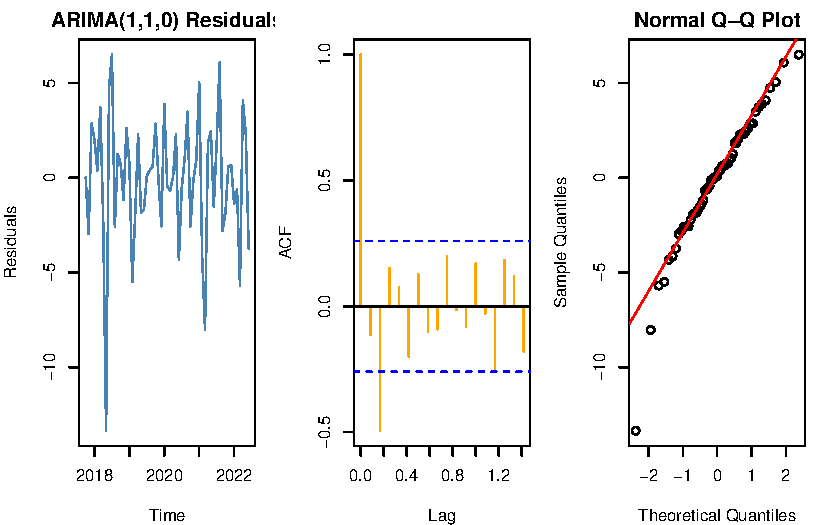
\includegraphics{project_files/figure-pdf/fig-ARIMA Model Fitting-1.pdf}

}

\caption{ARIMA Model Fitting}

\end{figure}%

\begin{figure}[H]

{\centering 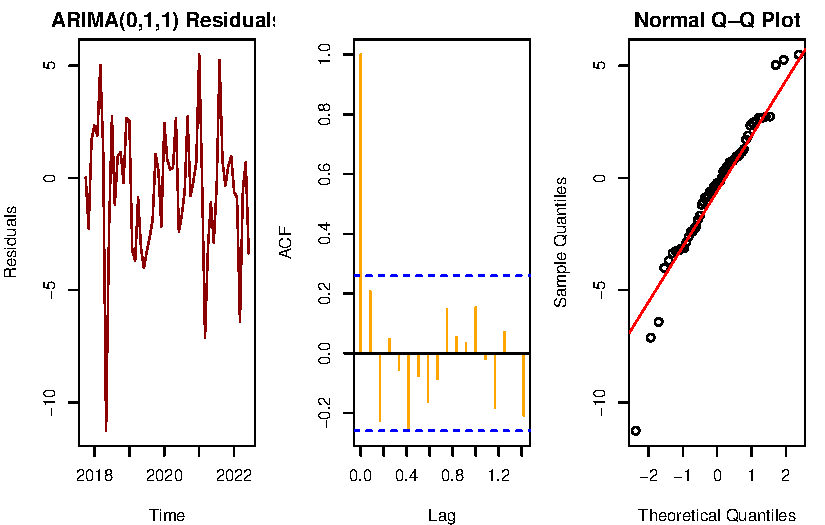
\includegraphics{project_files/figure-pdf/fig-ARIMA Model Fitting-2.pdf}

}

\caption{ARIMA Model Fitting}

\end{figure}%

\begin{figure}[H]

{\centering 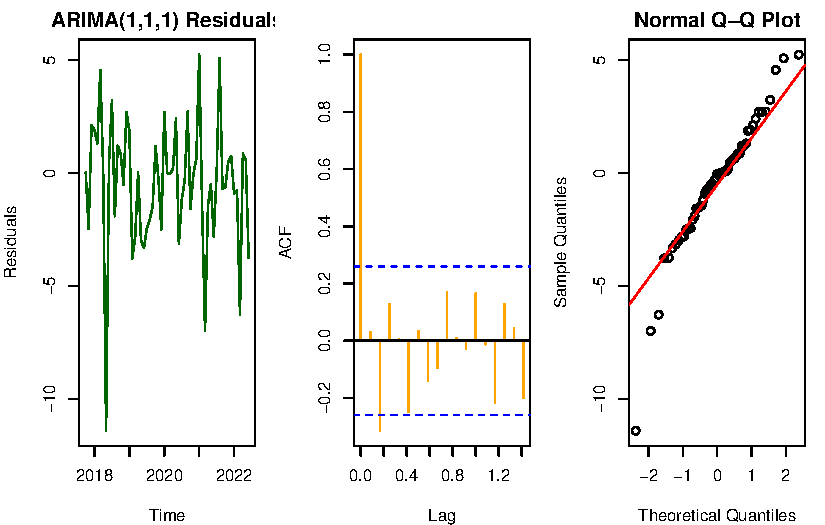
\includegraphics{project_files/figure-pdf/fig-ARIMA Model Fitting-3.pdf}

}

\caption{ARIMA Model Fitting}

\end{figure}%

\begin{verbatim}
ARIMA(1,1,0): AIC = 301.4389 , Ljung-Box p = 0.005049932 
\end{verbatim}

\begin{verbatim}
ARIMA(0,1,1): AIC = 286.6222 , Ljung-Box p = 0.1412433 
\end{verbatim}

\begin{verbatim}
ARIMA(1,1,1): AIC = 285.0751 , Ljung-Box p = 0.1265184 
\end{verbatim}




\end{document}
